\documentclass[11pt,a4paper]{article}

% Image mode: pdf.
% Image paths stay relative. In PDF mode, place same-basename PDF conversions
% of the chapter SVG files in the assets/ directory beside this source.

\usepackage{iftex}
\ifPDFTeX
  \PackageError{handout}{This template requires XeTeX or Tectonic}{Compile with xelatex or tectonic.}
\fi

\usepackage[a4paper,top=18mm,bottom=20mm,left=20mm,right=20mm,headsep=6mm]{geometry}
\usepackage{fontspec}
\usepackage{xeCJK}
\usepackage{amsmath}
\usepackage{unicode-math}

% Font settings are intentionally visible in the generated .tex file.
% These defaults target the macOS machine used for the released PDF.
% Change the family names when compiling on another system.
\setmainfont{Songti TC}
\setsansfont{Heiti TC}
\setmonofont{Menlo}
\setCJKmainfont{Songti TC}
\setCJKsansfont{Heiti TC}
\setCJKmonofont{Heiti TC}
\setmathfont{STIX Two Math}
\XeTeXlinebreaklocale "zh"
\XeTeXlinebreakskip=0pt plus 1pt

\usepackage{xcolor}
\definecolor{HandoutBlue}{HTML}{215A91}
\definecolor{HandoutBlueLight}{HTML}{EEF5FC}
\definecolor{HandoutGreen}{HTML}{39715A}
\definecolor{HandoutGreenLight}{HTML}{EFF8F3}
\definecolor{HandoutGold}{HTML}{8A641C}
\definecolor{HandoutGoldLight}{HTML}{FFF8E8}
\definecolor{HandoutInk}{HTML}{253142}
\definecolor{HandoutMuted}{HTML}{667085}

\usepackage{graphicx}
\makeatletter
% Pandoc 3 emits an accessibility `alt` key for raster/PDF images. Older
% graphicx releases do not know that key, so accept it without changing layout.
\@ifundefined{KV@Gin@alt}{\define@key{Gin}{alt}{}}{}
\newsavebox\pandoc@box
\newcommand*\pandocbounded[1]{%
  \sbox\pandoc@box{#1}%
  \Gscale@div\@tempa{\textheight}{\dimexpr\ht\pandoc@box+\dp\pandoc@box\relax}%
  \Gscale@div\@tempb{\linewidth}{\wd\pandoc@box}%
  \ifdim\@tempb\p@<\@tempa\p@\let\@tempa\@tempb\fi
  \ifdim\@tempa\p@<\p@\scalebox{\@tempa}{\usebox\pandoc@box}%
  \else\usebox{\pandoc@box}%
  \fi
}
\makeatother
\usepackage{float}
\floatplacement{figure}{H}
% Pandoc uses LTcaptype=none for uncaptioned longtables. The caption package
% expects that name to exist as a counter even though it is never displayed.
\newcounter{none}
\usepackage{caption}
\captionsetup[figure]{labelformat=empty,labelsep=none,font=small}

\usepackage{booktabs,longtable,array,calc}
\usepackage{etoolbox}
\makeatletter
\patchcmd\longtable{\par}{\if@noskipsec\mbox{}\fi\par}{}{}
\makeatother

\usepackage[most]{tcolorbox}
\tcbuselibrary{breakable,skins}
\newtcolorbox{HandoutLearningMap}{
  enhanced,breakable,colback=HandoutBlueLight,colframe=HandoutBlue,
  boxrule=0.8pt,arc=1.5mm,left=3mm,right=3mm,top=2mm,bottom=2mm,
  before skip=8pt,after skip=10pt
}
\newtcolorbox{HandoutWorkedExample}{
  enhanced,breakable,colback=HandoutGreenLight,colframe=HandoutGreen,
  boxrule=0.65pt,arc=1.5mm,left=3mm,right=3mm,top=2mm,bottom=2mm,
  before skip=8pt,after skip=10pt
}
\newtcolorbox{HandoutSelfCheck}{
  enhanced,breakable,colback=HandoutGoldLight,colframe=HandoutGold,
  boxrule=0.65pt,arc=1.5mm,left=3mm,right=3mm,top=2mm,bottom=2mm,
  before skip=8pt,after skip=10pt
}

\usepackage{titlesec}
\titleformat{\section}{\sffamily\bfseries\Large\color{HandoutBlue}}{}{0pt}{}
\titleformat{\subsection}{\sffamily\bfseries\large\color{HandoutInk}}{}{0pt}{}
\titleformat{\subsubsection}{\sffamily\bfseries\normalsize\color{HandoutInk}}{}{0pt}{}
\titlespacing*{\section}{0pt}{1.4em}{0.55em}
\titlespacing*{\subsection}{0pt}{1.15em}{0.45em}
\titlespacing*{\subsubsection}{0pt}{0.9em}{0.35em}
\setcounter{secnumdepth}{-\maxdimen}

\usepackage{hyperref}
\usepackage{bookmark}
\IfFileExists{xurl.sty}{\usepackage{xurl}}{}
\urlstyle{same}
\hypersetup{
  colorlinks=true,
  linkcolor=HandoutBlue,
  urlcolor=HandoutBlue,
  citecolor=HandoutBlue,
  pdftitle={選化II-2 物質的性質與化學鍵},
  pdfsubject={化學},
  pdfcreator={Pandoc with the HighSchooContent LaTeX template}
}

\setlength{\parindent}{0pt}
\setlength{\parskip}{0.55em plus 0.15em minus 0.1em}
\setlength{\emergencystretch}{3em}
\setlength{\LTpre}{0.5em}
\setlength{\LTpost}{0.5em}
\renewcommand{\arraystretch}{1.18}
\providecommand{\tightlist}{%
  \setlength{\itemsep}{0pt}\setlength{\parskip}{0pt}}
\pagestyle{plain}


\begin{document}

\begin{tcolorbox}[
  enhanced,colback=white,colframe=HandoutBlue,boxrule=1.1pt,arc=2mm,
  borderline west={3pt}{0pt}{HandoutBlue},left=5mm,right=4mm,top=4mm,bottom=4mm
]
{\sffamily\small\bfseries\color{HandoutBlue}學生講義}\par
{\sffamily\bfseries\LARGE\color{HandoutInk}選化II-2 物質的性質與化學鍵}\par
\vspace{0.35em}{\large 由粒子之間的吸引、軌域重疊、分子形狀與電荷分布，推得材料性質、分子極性與沸點}\par
\vspace{0.45em}{\small\color{HandoutMuted}%
科目：化學
\quad 課程：普通高中選修化學 II
\quad 版本：學生版｜核心＋理解
\quad 校訂：2026-08-29
}\par
\vspace{0.25em}{\small\color{HandoutMuted}範圍：現行選修化學 II 第二章主線；涵蓋化學鍵種類、單鍵與多鍵、sp3／sp2／sp 混成、VSEPR、鍵與分子極性、分子間作用力；五、六電子域形狀僅列為理解延伸}\par
\end{tcolorbox}


同一批元素可以形成食鹽、銅線、石墨與塑膠，性質差異來自粒子的連接方式。先辨認構成粒子與化學鍵，再由軌域重疊建立單鍵、多鍵與混成模型；分子形成後，還需把三維形狀與各鍵的電荷偏移合成，才能判斷分子極性。最後比較分子間作用力，便能解釋熔、沸點、黏度、溶解與材料選擇。

\begin{HandoutLearningMap}

\subsection{本章問題與能力}\label{ux672cux7ae0ux554fux984cux8207ux80fdux529b}

\begin{enumerate}
\def\labelenumi{\arabic{enumi}.}
\tightlist
\item
  離子鍵、金屬鍵、共價鍵與共價網狀結構如何由粒子模型區分？
\item
  電荷、離子距離、軌域重疊與核間距如何改變鍵結穩定性？
\item
  單鍵、雙鍵與三鍵各含多少個 \(\sigma\) 鍵與 \(\pi\) 鍵？鍵級如何影響鍵長、鍵能與轉動？
\item
  \(sp^3\)、\(sp^2\)、\(sp\) 混成如何連接軌域數、成鍵方向與 \(\pi\) 鍵數？
\item
  如何由 Lewis 結構、電子域與 AX\(_m\)E\(_n\) 記號判斷分子形狀與鍵角？
\item
  鍵極性如何以向量合成為分子極性？分子間作用力如何決定沸點與溶解性？
\end{enumerate}

\end{HandoutLearningMap}

\section{1. 化學鍵的種類}\label{ux5316ux5b78ux9375ux7684ux7a2eux985e}

\subsection{1.1 鍵結的能量判準}\label{ux9375ux7d50ux7684ux80fdux91cfux5224ux6e96}

\textbf{化學鍵}是原子或離子之間足以形成穩定聚集體的淨吸引作用。兩粒子靠近時，同時存在核---電子吸引、核---核排斥與電子---電子排斥。核間距 \(r\) 改變時，這些作用的總和形成位能曲線 \(U(r)\)。

\begin{figure}
\centering
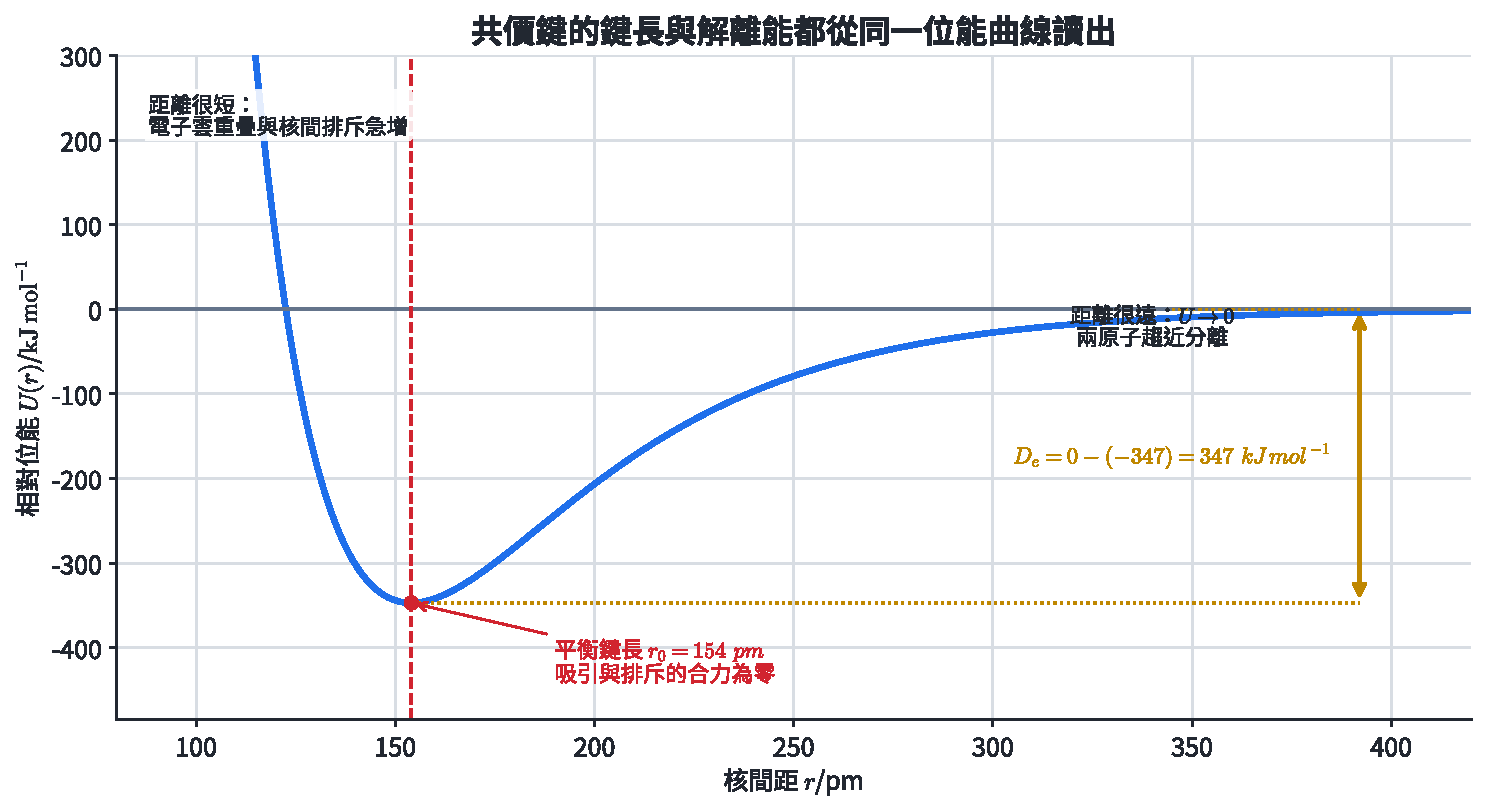
\includegraphics[width=0.94\linewidth,height=\textheight,keepaspectratio,alt={圖 1｜沿曲線由右向左讀：原子由遠處靠近時位能先下降，在 r\_0 最低；再壓近時排斥使位能急升。解離能是最低點到 U=0 的垂直能量差。}]{assets/選化II-2-共價鍵能量與鍵長.pdf}
\caption{圖 1｜沿曲線由右向左讀：原子由遠處靠近時位能先下降，在 \(r_0\) 最低；再壓近時排斥使位能急升。解離能是最低點到 \(U=0\) 的垂直能量差。}
\end{figure}

圖 1 的最低點滿足兩個條件：

\begin{itemize}
\tightlist
\item
  \(r=r_0\) 時位能最低，稱為\textbf{平衡鍵長}。
\item
  曲線斜率 \(\mathrm dU/\mathrm dr=0\)，因此吸引與排斥的合力為零。
\end{itemize}

由最低點把兩原子分開到 \(r\to\infty\)，需輸入的能量稱為\textbf{鍵解離能}。成鍵時沿相反路徑下降到最低點，系統釋放相同量級的能量。鍵長描述穩定距離；鍵能描述離開最低點所需能量，兩者是不同物理量。

\subsection{1.2 離子鍵與離子晶體}\label{ux96e2ux5b50ux9375ux8207ux96e2ux5b50ux6676ux9ad4}

正、負離子之間的靜電吸引稱為\textbf{離子鍵}。離子晶體由大量離子週期排列，每一個離子同時受周圍多個異號離子吸引，也受同號離子排斥；整個晶格的總靜電位能決定穩定性。離子鍵不指定一對原子的固定方向，因此稱為非方向性作用。

比較相同晶格型式的離子化合物時，可用庫侖作用的量級判斷：

\[
|U|\propto \frac{|z_+z_-|}{r},
\]

其中 \(z_+\)、\(z_-\) 是離子電荷數，\(r\) 是正負離子的最近鄰距離。電荷乘積越大、距離越短，靜電吸引通常越強。

本章把\textbf{晶格能大小}定義為：一莫耳離子晶體完全分離成氣態離子所需的能量，數值取正。若資料把氣態離子形成晶體的能量變化寫成負值，兩者絕對值相同、符號相反；作答時需先讀清楚定義。

\begin{figure}
\centering
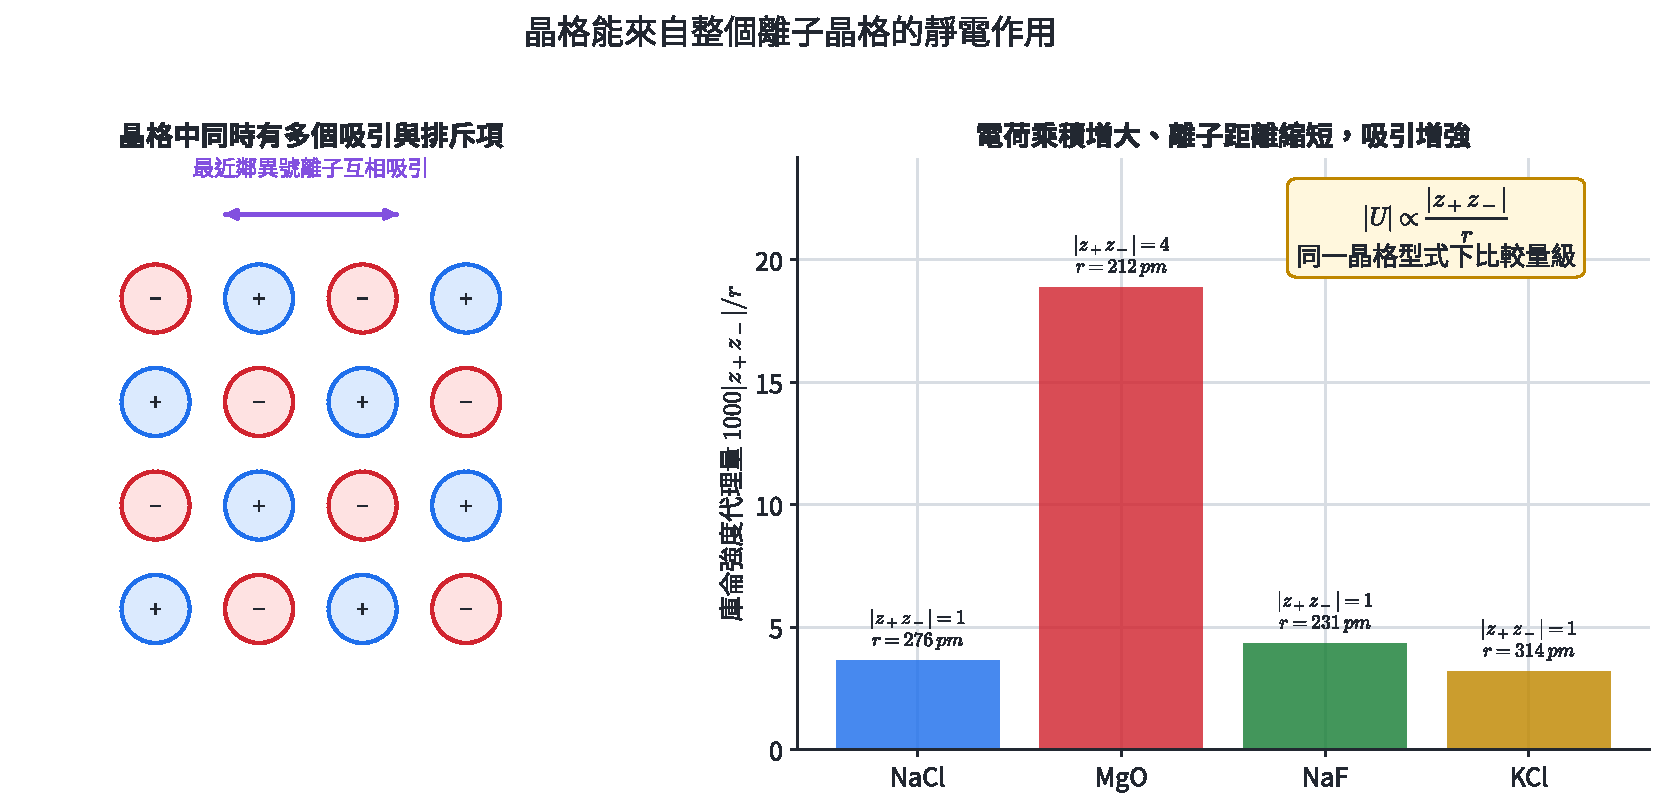
\includegraphics[width=0.96\linewidth,height=\textheight,keepaspectratio,alt={圖 2｜左圖的正負離子數相等；右圖以電荷乘積除以距離比較四組離子的庫侖作用量級。}]{assets/選化II-2-離子晶格與晶格能.pdf}
\caption{圖 2｜左圖的正負離子數相等；右圖以電荷乘積除以距離比較四組離子的庫侖作用量級。}
\end{figure}

離子晶體的常見性質可由結構直接推得：

\begin{itemize}
\tightlist
\item
  晶格中離子受多方向吸引，熔化需破壞大量靜電作用，熔點通常較高。
\item
  固態離子被固定在晶格位置，難以形成定向電流；熔融或溶於水後，離子可移動，便能導電。
\item
  受力使晶格層滑移時，同號離子可能相鄰而強烈排斥，因此常呈脆性。
\end{itemize}

\subsection{1.3 金屬鍵與金屬晶體}\label{ux91d1ux5c6cux9375ux8207ux91d1ux5c6cux6676ux9ad4}

金屬可用「金屬陽離子骨架與離域價電子互相吸引」描述。價電子分布於整個晶體，沒有固定屬於某一對原子，這種非方向性的吸引稱為\textbf{金屬鍵}。

\begin{figure}
\centering
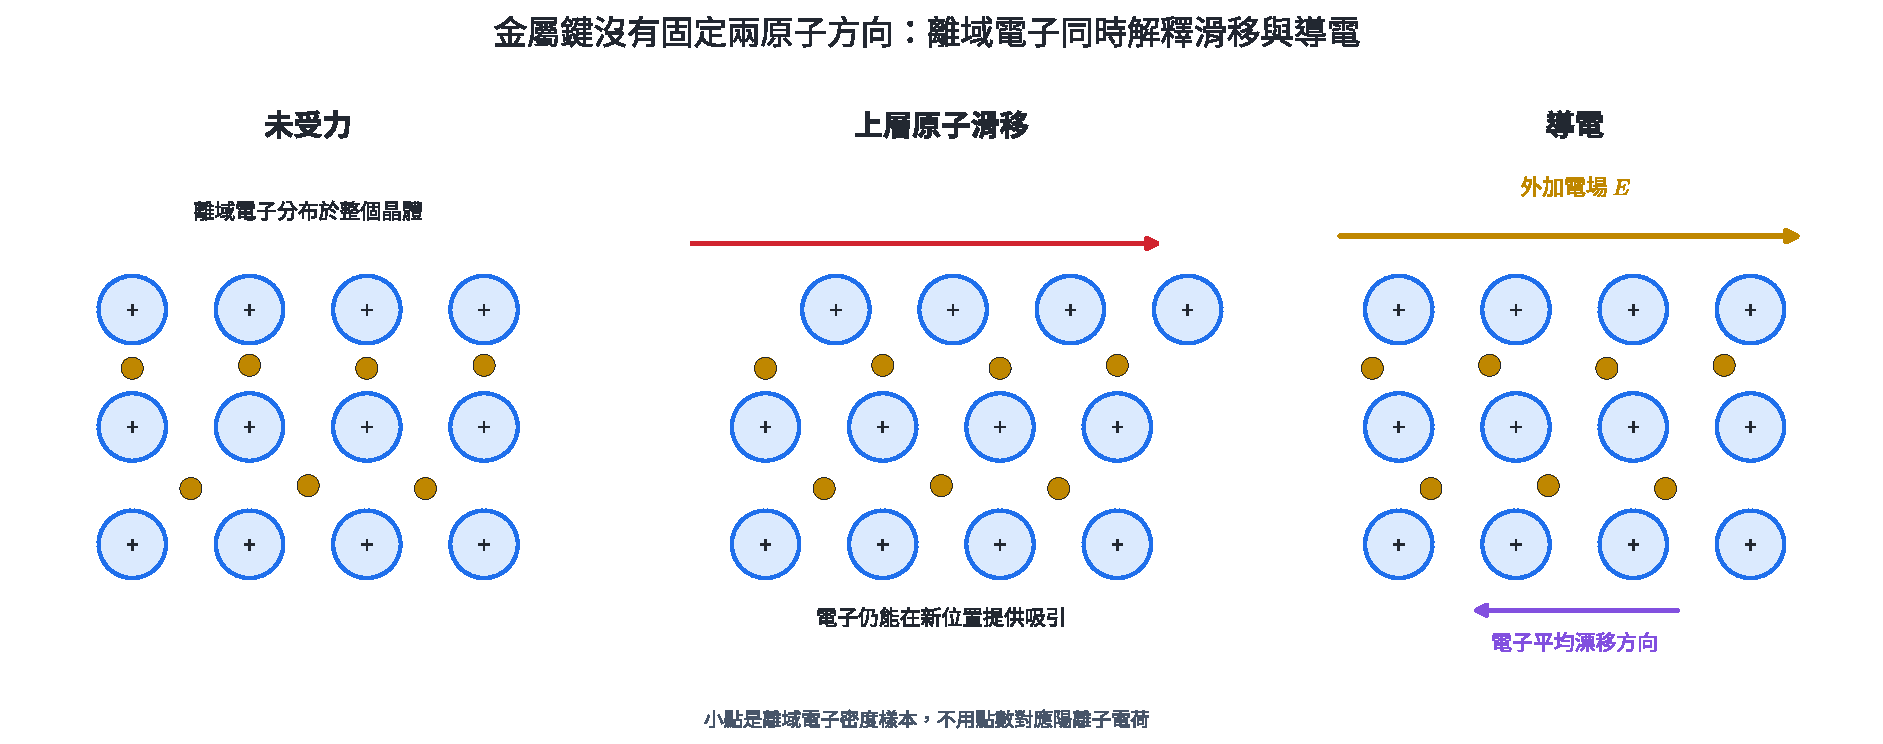
\includegraphics[width=0.96\linewidth,height=\textheight,keepaspectratio,alt={圖 3｜晶格層滑移後，離域電子仍可提供吸引；外加電場時，電子平均漂移方向與電場方向相反。小點代表電子密度樣本。}]{assets/選化II-2-金屬鍵與材料變形.pdf}
\caption{圖 3｜晶格層滑移後，離域電子仍可提供吸引；外加電場時，電子平均漂移方向與電場方向相反。小點代表電子密度樣本。}
\end{figure}

圖 3 同時解釋兩項性質：

\begin{itemize}
\tightlist
\item
  金屬層滑移時，離域電子可重新分布並維持吸引，因此金屬可延展、壓成薄片或拉成線。
\item
  電子可在晶體內移動；施加電場後產生平均漂移，因此金屬通常導電。
\end{itemize}

電子海模型足以連結結構、導電與延展性。不同金屬的導電度、磁性與半導體能隙需進一步使用能帶模型；高中層次把能帶視為電子可用能量範圍即可。

\subsection{1.4 共價鍵、分子物質與共價網狀固體}\label{ux5171ux50f9ux9375ux5206ux5b50ux7269ux8ceaux8207ux5171ux50f9ux7db2ux72c0ux56faux9ad4}

兩原子的價軌域沿特定方向重疊，共用電子密度集中在兩核之間，使總位能下降，形成\textbf{共價鍵}。軌域重疊有明確空間方向，因此共價鍵具有方向性。

共價鍵可形成兩類不同尺度的物質：

\begin{enumerate}
\def\labelenumi{\arabic{enumi}.}
\tightlist
\item
  \textbf{分子物質}：原子先以共價鍵形成獨立分子；熔化、沸騰主要克服分子間作用力，不必逐一切斷分子內共價鍵。
\item
  \textbf{共價網狀固體}：原子以共價鍵連成整個晶體，例如鑽石、石英 \(\mathrm{SiO_2}\) 與碳化矽。熔化或變形需改變廣泛的共價鍵，通常硬且熔點高。
\end{enumerate}

石墨是重要的結構---性質例外：每個碳原子在同一層與三個碳成鍵，層內有可移動的離域電子，因此沿層面可導電；層與層之間作用較弱，容易相對滑動，所以可作鉛筆芯與固體潤滑材料。

\begin{figure}
\centering
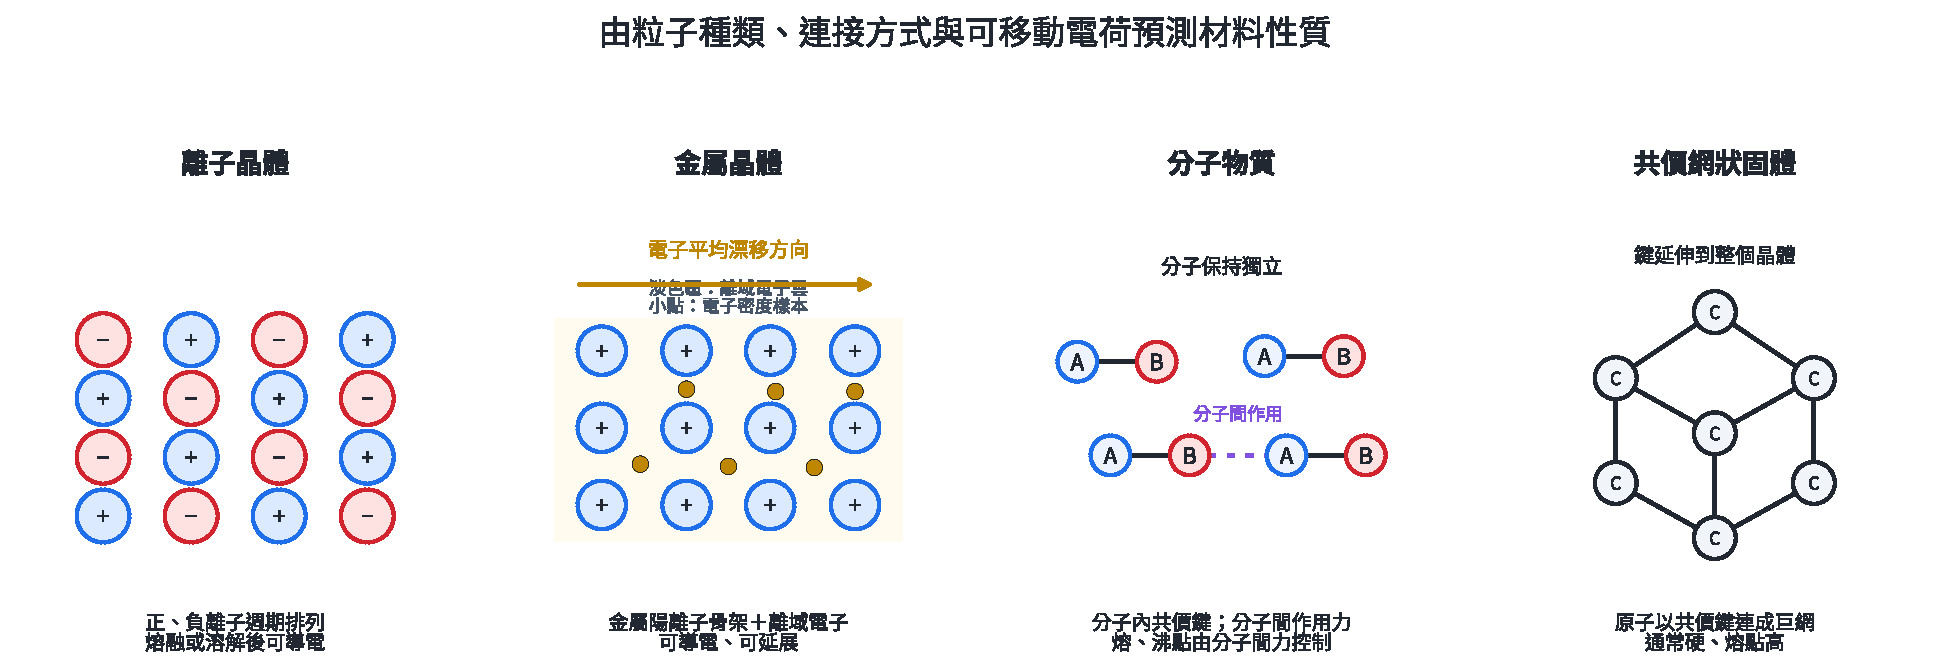
\includegraphics[width=0.98\linewidth,height=\textheight,keepaspectratio,alt={圖 4｜先看粒子是離子、金屬陽離子、獨立分子或共價網，再由可移動電荷與連接範圍預測性質。金屬圖的小點是電子密度樣本；分子圖的虛線連接兩個實際分子。}]{assets/選化II-2-鍵結模型與材料性質.pdf}
\caption{圖 4｜先看粒子是離子、金屬陽離子、獨立分子或共價網，再由可移動電荷與連接範圍預測性質。金屬圖的小點是電子密度樣本；分子圖的虛線連接兩個實際分子。}
\end{figure}

\begin{HandoutWorkedExample}

\subsection{示範 1｜由電荷與距離比較晶格吸引}\label{ux793aux7bc4-1ux7531ux96fbux8377ux8207ux8dddux96e2ux6bd4ux8f03ux6676ux683cux5438ux5f15}

以 \(|z_+z_-|/r\) 作量級比較。已知最近鄰距離：NaCl 為 \(276\ \mathrm{pm}\)，MgO 為 \(212\ \mathrm{pm}\)。判斷哪一晶格的靜電吸引較強。

NaCl 中 \(|z_+z_-|=1\)：

\[
S_{\mathrm{NaCl}}=\frac{1}{276}=3.62\times10^{-3}\ \mathrm{pm^{-1}}.
\]

MgO 中 \(|z_+z_-|=|(+2)(-2)|=4\)：

\[
S_{\mathrm{MgO}}=\frac{4}{212}=1.89\times10^{-2}\ \mathrm{pm^{-1}}.
\]

比值為

\[
\frac{S_{\mathrm{MgO}}}{S_{\mathrm{NaCl}}}=5.22.
\]

在晶格型式與其他因素相近的比較下，MgO 的靜電吸引量級較大，因此通常有較大的晶格能與較高熔點。這個比例只用來判斷趨勢；精確晶格能還取決於完整三維排列與排斥項。

\end{HandoutWorkedExample}

\begin{HandoutWorkedExample}

\subsection{示範 2｜由性質資料反推固體結構}\label{ux793aux7bc4-2ux7531ux6027ux8ceaux8cc7ux6599ux53cdux63a8ux56faux9ad4ux7d50ux69cb}

三種固體的資料如下。

{\def\LTcaptype{none} % do not increment counter
\begin{longtable}[]{@{}lrrrr@{}}
\toprule\noalign{}
固體 & 熔點 & 固態導電 & 熔融導電 & 可延展 \\
\midrule\noalign{}
\endhead
\bottomrule\noalign{}
\endlastfoot
P & 高 & 否 & 是 & 否 \\
Q & 高 & 是 & 是 & 是 \\
R & 低 & 否 & 否 & 否 \\
\end{longtable}
}

判斷 P、Q、R 最可能的結構類型。

P 固態不導電而熔融導電，表示帶電粒子固態時被固定、熔融後可移動；P 最符合離子晶體。Q 在固、液態都導電且可延展，表示有可移動電子且鍵結可隨滑移重組；Q 最符合金屬晶體。R 熔點低且兩狀態都不導電，表示由中性獨立分子組成；R 最符合分子物質。

資料若只有「熔點高」仍不足以區分離子晶體、金屬晶體與共價網狀固體；加入載流子能否移動與機械性質後，判斷才有辨識力。

\end{HandoutWorkedExample}

\begin{HandoutWorkedExample}

\subsection{示範 3｜鑽石與石墨皆由碳組成，性質為何不同}\label{ux793aux7bc4-3ux947dux77f3ux8207ux77f3ux58a8ux7686ux7531ux78b3ux7d44ux6210ux6027ux8ceaux70baux4f55ux4e0dux540c}

鑽石中每個碳以四個共價鍵連成立體網路。局部變形會牽動多方向的強鍵，因此鑽石硬；電子局域於鍵結，常溫下缺少可移動載流子，因此不易導電。

石墨中每個碳在平面內與三個碳成鍵，剩餘電子形成層內離域系統，因此沿層面導電。層間作用遠弱於層內共價鍵，外力可使各層滑移，所以石墨柔軟並可留下痕跡。

元素組成相同只保證原子種類相同；連接數、維度與電子能否離域才直接控制材料性質。

\end{HandoutWorkedExample}

\subsection{1.5 直接用途與材料判讀}\label{ux76f4ux63a5ux7528ux9014ux8207ux6750ux6599ux5224ux8b80}

電線需要導電與延展，金屬鍵模型可解釋銅與鋁的選用；耐磨刀具需要三維強鍵網路，鑽石與碳化矽符合此條件；電解質感測器利用離子在溶液中的移動；耐火陶瓷則利用離子晶格或共價網狀結構的高鍵結能。工程選材仍需同時考慮密度、成本、氧化與缺陷，本章模型提供第一層結構判斷。

\subsection{練習 1}\label{ux7df4ux7fd2-1}

\begin{enumerate}
\def\labelenumi{\arabic{enumi}.}
\tightlist
\item
  已知 NaF 與 NaCl 的離子電荷相同，最近鄰距離分別為 \(231\ \mathrm{pm}\)、\(276\ \mathrm{pm}\)。用庫侖量級比較兩者的晶格吸引。
\item
  CaO 與 KCl 的最近鄰距離均近似為 \(280\ \mathrm{pm}\)。比較 \(|z_+z_-|/r\)，判斷何者晶格吸引較強。
\item
  某固體熔點高，固態不導電，熔融後導電，受撞擊易碎。寫出最可能的結構與四項性質的粒子層次原因。
\item
  銅可拉成細線且可導電。各用一句微觀敘述連接金屬鍵模型與這兩項性質。
\item
  比較乾冰與石英：兩者都含非金屬元素，為何乾冰易昇華而石英熔點高？
\item
  某黑色碳材料沿薄片方向導電且容易剝成薄層。根據結構---性質證據判斷較接近鑽石或石墨，並說明兩項證據。
\end{enumerate}

\subsection{練習 1 解析}\label{ux7df4ux7fd2-1-ux89e3ux6790}

\begin{enumerate}
\def\labelenumi{\arabic{enumi}.}
\item
  電荷乘積相同時 \(|U|\propto1/r\)：

  \[
  \frac{S_{\mathrm{NaF}}}{S_{\mathrm{NaCl}}}=\frac{276}{231}=1.19.
  \]

  NaF 的庫侖吸引量級約為 NaCl 的 \(1.19\) 倍。
\item
  KCl 的電荷乘積為 \(1\)；CaO 為 \(4\)。距離相同時 CaO 的量級約為 KCl 的 \(4\) 倍。
\item
  最可能是離子晶體。高熔點來自廣泛靜電吸引；固態離子被固定而不導電；熔融後離子可移動而導電；晶格層錯開會使同號離子相鄰、排斥增大而斷裂。
\item
  延展：原子層滑移後離域電子重新分布並維持吸引。導電：外加電場使離域電子出現平均漂移。
\item
  乾冰由獨立 \(\mathrm{CO_2}\) 分子組成，昇華主要克服分子間作用力；石英的 Si、O 原子以共價鍵連成巨網，熔化需改變大量強鍵。
\item
  較接近石墨。沿片導電對應層內離域電子；容易剝層對應層間作用弱。鑽石是三維網路且缺少這類層狀滑移。
\end{enumerate}

\section{2. 單鍵與多鍵}\label{ux55aeux9375ux8207ux591aux9375}

\subsection{\texorpdfstring{2.1 \(\sigma\) 鍵與 \(\pi\) 鍵}{2.1 \textbackslash sigma 鍵與 \textbackslash pi 鍵}}\label{sigma-ux9375ux8207-pi-ux9375}

兩原子軌域沿核間軸迎面重疊，電子密度集中在核間軸附近，形成 \textbf{\(\sigma\) 鍵}。兩個平行的未混成 \(p\) 軌域在核間軸兩側側向重疊，形成 \textbf{\(\pi\) 鍵}。

對同一對相連原子：

\[
\begin{aligned}
\text{單鍵}&=1\sigma,\\
\text{雙鍵}&=1\sigma+1\pi,\\
\text{三鍵}&=1\sigma+2\pi.
\end{aligned}
\]

每對相連原子只有一個 \(\sigma\) 鍵；增加的鍵級由 \(\pi\) 鍵提供。\(\sigma\) 重疊沿核間軸，通常比單一 \(\pi\) 側向重疊強。雙鍵總能量高於單鍵，但不等於兩個單鍵能量；三鍵也不等於三倍單鍵能量。

\begin{figure}
\centering
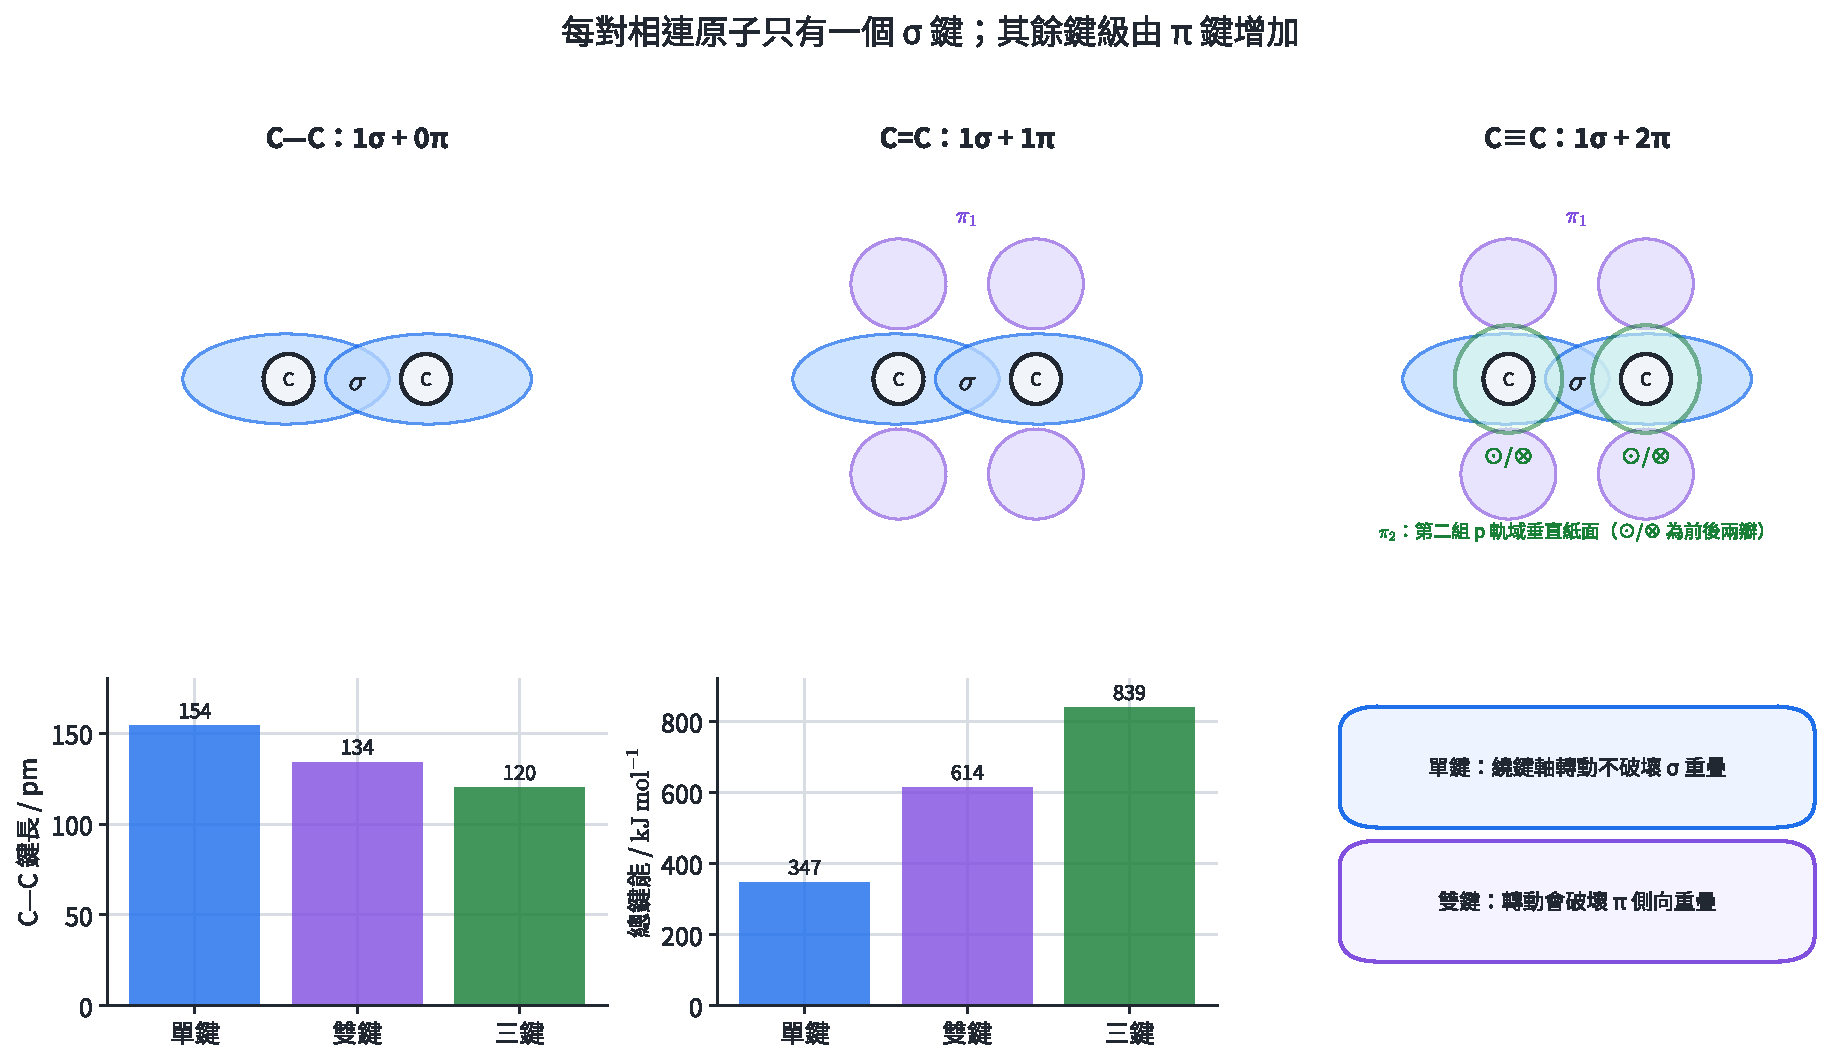
\includegraphics[width=0.98\linewidth,height=\textheight,keepaspectratio,alt={圖 5｜上排由軌域重疊數出 \textbackslash sigma、\textbackslash pi；三鍵中的 \textbackslash odot/\textbackslash otimes 表示每個 C 的第二組 p 軌域在紙面前後的兩瓣。下排標出同一組 C---C 鍵長與總鍵能數值。}]{assets/選化II-2-單鍵多鍵與sigma-pi.pdf}
\caption{圖 5｜上排由軌域重疊數出 \(\sigma\)、\(\pi\)；三鍵中的 \(\odot/\otimes\) 表示每個 C 的第二組 \(p\) 軌域在紙面前後的兩瓣。下排標出同一組 C---C 鍵長與總鍵能數值。}
\end{figure}

\subsection{2.2 鍵級、鍵長、鍵能與轉動}\label{ux9375ux7d1aux9375ux9577ux9375ux80fdux8207ux8f49ux52d5}

同種原子形成的鍵可用\textbf{鍵級}表示共用電子對數。C---C、C=C、C\(\equiv\)C 的鍵級依序為 \(1,2,3\)。鍵級增加時，核間電子密度增加，穩定距離通常縮短，切斷全部鍵所需的總能量通常增加：

\[
r_{\mathrm{C\equiv C}}<r_{\mathrm{C=C}}<r_{\mathrm{C-C}},
\]

\[
D_{\mathrm{C\equiv C}}>D_{\mathrm{C=C}}>D_{\mathrm{C-C}}.
\]

繞單一 \(\sigma\) 鍵軸轉動時，迎面重疊大致維持；繞雙鍵轉動會使兩個 \(p\) 軌域失去平行，破壞 \(\pi\) 重疊。因此雙鍵限制自由轉動，順反異構與聚合物構型便由此產生。

\subsection{2.3 由平均鍵能估算反應熱}\label{ux7531ux5e73ux5747ux9375ux80fdux4f30ux7b97ux53cdux61c9ux71b1}

氣相分子的平均鍵能可用來估算反應焓：

\[
\Delta H\approx \sum D(\text{斷鍵})-\sum D(\text{成鍵}).
\]

斷鍵需輸入能量，列正項；成鍵釋放能量，列負項。平均鍵能把不同分子環境中的同類鍵取平均，因此結果是估計值；精確反應焓需使用各物質的標準生成焓。

\begin{HandoutWorkedExample}

\subsection{\texorpdfstring{示範 4｜數出分子中的 \(\sigma\) 鍵與 \(\pi\) 鍵}{示範 4｜數出分子中的 \textbackslash sigma 鍵與 \textbackslash pi 鍵}}\label{ux793aux7bc4-4ux6578ux51faux5206ux5b50ux4e2dux7684-sigma-ux9375ux8207-pi-ux9375}

求 \(\mathrm{CH_2=CH-C\equiv N}\) 中 \(\sigma\)、\(\pi\) 鍵數。

先數相連原子對，每一對給一個 \(\sigma\) 鍵：四個 C---H、C\(_1\)---C\(_2\)、C\(_2\)---C\(_3\)、C\(_3\)---N，共

\[
N_\sigma=4+3=7.
\]

再數多鍵增加的 \(\pi\)：一個 C=C 含 \(1\pi\)，一個 C\(\equiv\)N 含 \(2\pi\)，所以

\[
N_\pi=1+2=3.
\]

檢查：雙鍵的鍵級 \(2=1\sigma+1\pi\)，三鍵的鍵級 \(3=1\sigma+2\pi\)；沒有把多鍵中的 \(\sigma\) 重複計數。

\end{HandoutWorkedExample}

\begin{HandoutWorkedExample}

\subsection{示範 5｜用鍵能估算氫化反應熱}\label{ux793aux7bc4-5ux7528ux9375ux80fdux4f30ux7b97ux6c2bux5316ux53cdux61c9ux71b1}

估算

\[
\mathrm{C_2H_4(g)+H_2(g)\rightarrow C_2H_6(g)}
\]

的 \(\Delta H\)。取 \(D(\mathrm{C=C})=614\)、\(D(\mathrm{H-H})=436\)、\(D(\mathrm{C-C})=347\)、\(D(\mathrm{C-H})=413\ \mathrm{kJ\,mol^{-1}}\)。

反應前後相同的四個 C---H 不必同時拆、同時建。淨變化是斷一個 C=C 與一個 H---H，形成一個 C---C 與兩個新 C---H：

\[
\begin{aligned}
\Delta H
&\approx[614+436]-[347+2(413)]\\
&=-123\ \mathrm{kJ\,mol^{-1}}.
\end{aligned}
\]

負號表示成鍵釋放的能量大於斷鍵吸收的能量，反應為放熱。這也說明雙鍵雖較強，加入 H\(_2\) 後形成一個 \(\sigma\) C---C 與兩個 C---H 的總穩定化更大。

\end{HandoutWorkedExample}

\subsection{2.4 直接用途}\label{ux76f4ux63a5ux7528ux9014}

雙鍵限制轉動，使天然橡膠、脂肪酸與視黃醛具有可辨認的幾何構型；加成聚合把 C=C 的 \(\pi\) 鍵轉成新的 \(\sigma\) 鍵，連成聚乙烯等長鏈。平均鍵能可快速估算燃燒、氫化與材料反應的放熱量，用於判斷熱管理方向；工程計算仍需實測熱化學資料。

\subsection{練習 2}\label{ux7df4ux7fd2-2}

\begin{enumerate}
\def\labelenumi{\arabic{enumi}.}
\tightlist
\item
  寫出 N---N、N=N、N\(\equiv\)N 各含多少個 \(\sigma\)、\(\pi\) 鍵。
\item
  求 \(\mathrm{CH_3-CH=CH-C\equiv CH}\) 的 \(\sigma\)、\(\pi\) 鍵總數。
\item
  已知 C---C、C=C、C\(\equiv\)C 鍵長分別為 \(154,134,120\ \mathrm{pm}\)。將三者按鍵級、鍵長與總鍵能由小到大排序。
\item
  乙烷可繞 C---C 鍵改變構形；乙烯的 C=C 使旋轉受限。用軌域重疊說明差異。
\item
  取 \(D(\mathrm{H-H})=436\)、\(D(\mathrm{Cl-Cl})=243\)、\(D(\mathrm{H-Cl})=431\ \mathrm{kJ\,mol^{-1}}\)，估算 \(\mathrm{H_2+Cl_2\rightarrow2HCl}\) 的 \(\Delta H\)。
\item
  某反應估算得 \(\sum D(\text{斷鍵})=1260\ \mathrm{kJ\,mol^{-1}}\)、\(\sum D(\text{成鍵})=1440\ \mathrm{kJ\,mol^{-1}}\)。求 \(\Delta H\)，說明放熱或吸熱，並指出平均鍵能法的一項限制。
\end{enumerate}

\subsection{練習 2 解析}\label{ux7df4ux7fd2-2-ux89e3ux6790}

\begin{enumerate}
\def\labelenumi{\arabic{enumi}.}
\item
  N---N：\(1\sigma,0\pi\)；N=N：\(1\sigma,1\pi\)；N\(\equiv\)N：\(1\sigma,2\pi\)。
\item
  相連原子對有 6 個 C---H 與 4 個 C---C，共 \(10\sigma\)；一個雙鍵與一個三鍵給 \(1+2=3\pi\)。
\item
  鍵級：單鍵 \(<\) 雙鍵 \(<\) 三鍵；鍵長：三鍵 \(<\) 雙鍵 \(<\) 單鍵；總鍵能：單鍵 \(<\) 雙鍵 \(<\) 三鍵。
\item
  乙烷的 C---C 只有沿鍵軸的 \(\sigma\) 重疊，繞軸旋轉仍能維持重疊。乙烯還有兩個平行 \(p\) 軌域的側向 \(\pi\) 重疊；旋轉會使其失去平行並需輸入破壞 \(\pi\) 鍵的能量。
\item
  \[
  \Delta H\approx(436+243)-2(431)=-183\ \mathrm{kJ\,mol^{-1}}.
  \]

  反應放熱。
\item
  \[
  \Delta H\approx1260-1440=-180\ \mathrm{kJ\,mol^{-1}}.
  \]

  負值表示放熱。平均鍵能是多種分子環境的平均，且通常以氣相鍵為基準，所以不能取代精確生成焓資料。
\end{enumerate}

\section{3. 混成軌域}\label{ux6df7ux6210ux8eccux57df}

\subsection{3.1 混成模型的目的與守恆}\label{ux6df7ux6210ux6a21ux578bux7684ux76eeux7684ux8207ux5b88ux6046}

同一原子的價層 \(s\)、\(p\) 軌域可以線性組合，建立一組方向與能量更適合描述局域鍵的\textbf{混成軌域}。混成前後遵守兩項帳目：

\begin{itemize}
\tightlist
\item
  參與組合的原子軌域數等於生成的混成軌域數。
\item
  混成只改變描述基底，價電子總數不變。
\end{itemize}

碳的價層含一個 \(2s\) 與三個 \(2p\) 軌域，共四個軌域。依成鍵環境，可建立：

\[
\begin{array}{c|c|c|c|c}
\text{混成} & \text{組合的軌域數} & \text{混成軌域數} & \text{未混成 }p\text{ 數} & \text{理想方向}\\ \hline
sp^3 & \text{1 個 }s+\text{3 個 }p & 4 & 0 & \text{四面體，}109.5^\circ\\
sp^2 & \text{1 個 }s+\text{2 個 }p & 3 & 1 & \text{平面三角，}120^\circ\\
sp & \text{1 個 }s+\text{1 個 }p & 2 & 2 & \text{直線，}180^\circ
\end{array}
\]

\begin{figure}
\centering
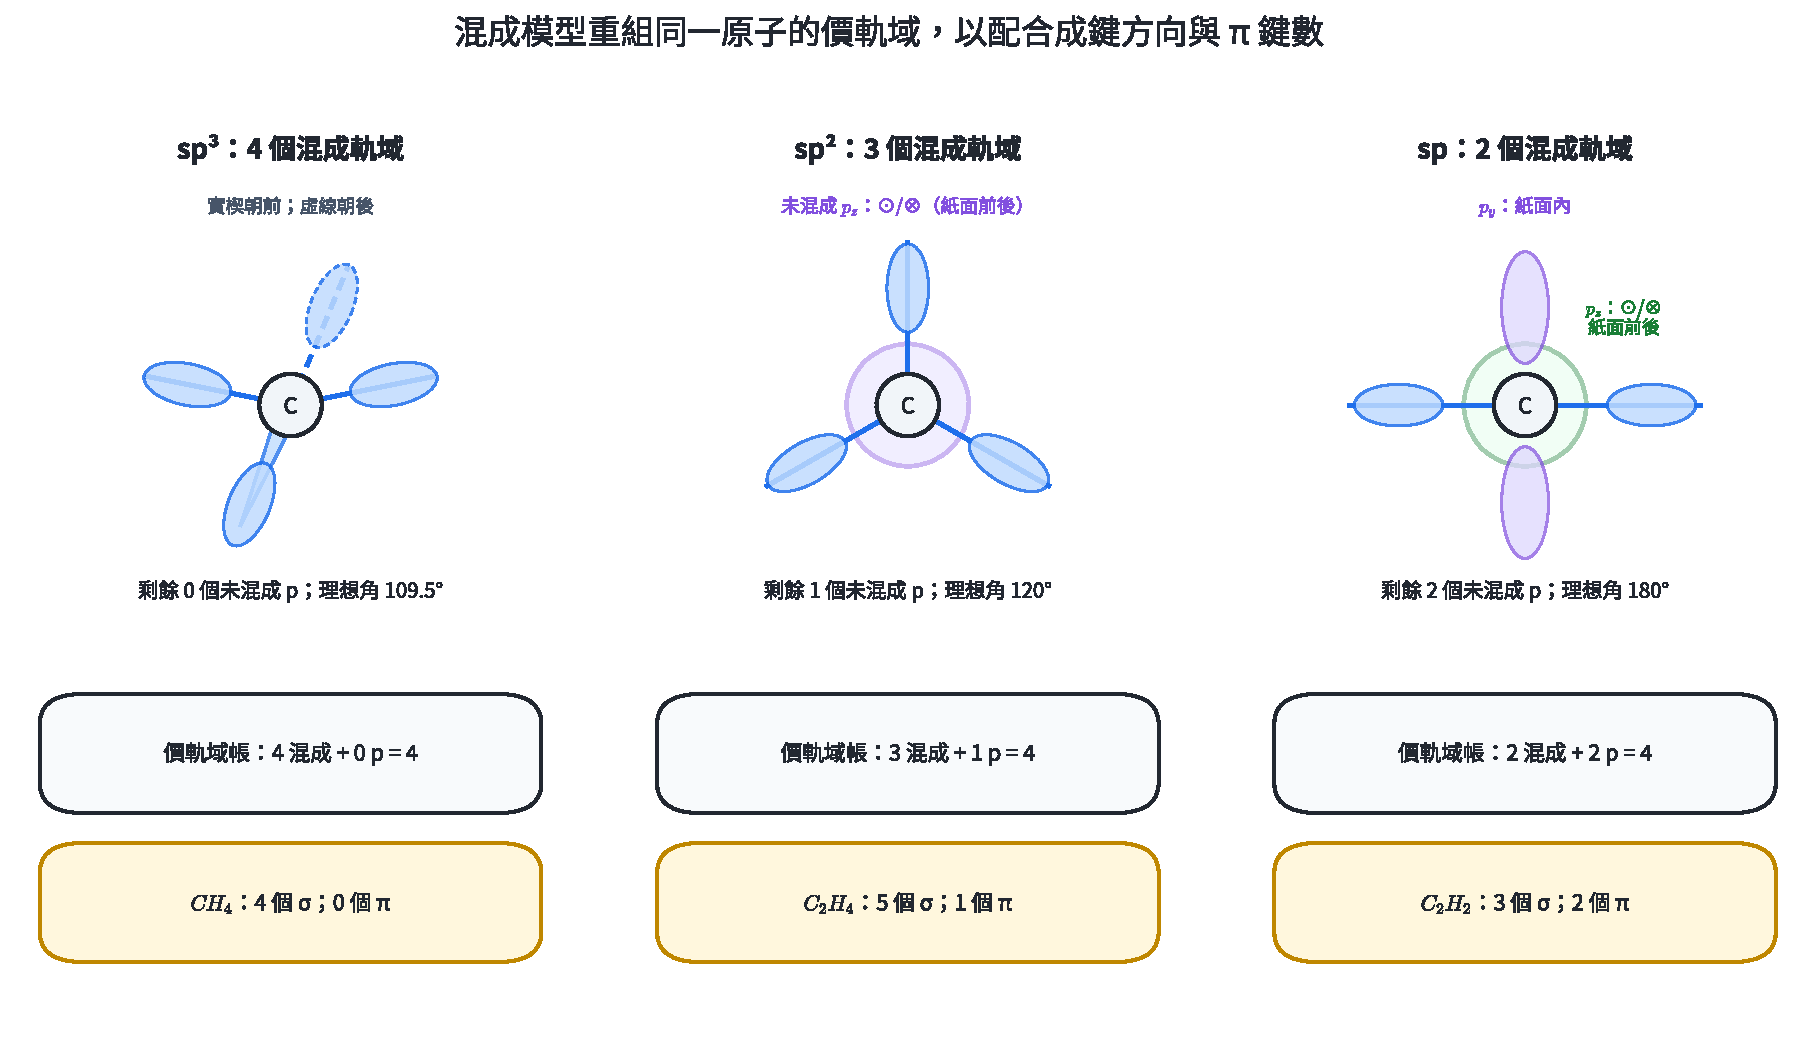
\includegraphics[width=0.98\linewidth,height=\textheight,keepaspectratio,alt={圖 6｜每欄先核對「混成軌域＋剩餘 p＝4」，再由剩餘 p 數連到 \textbackslash pi 鍵數與分子幾何。sp\^{}2 的剩餘 p\_z 垂直平面；sp 的 p\_y、p\_z 互相垂直，也都垂直鍵軸。}]{assets/選化II-2-sp3-sp2-sp混成模型.pdf}
\caption{圖 6｜每欄先核對「混成軌域＋剩餘 p＝4」，再由剩餘 p 數連到 \(\pi\) 鍵數與分子幾何。sp\(^2\) 的剩餘 \(p_z\) 垂直平面；sp 的 \(p_y\)、\(p_z\) 互相垂直，也都垂直鍵軸。}
\end{figure}

混成軌域主要形成 \(\sigma\) 鍵或容納孤電子對；未混成且彼此平行的 \(p\) 軌域才形成 \(\pi\) 鍵。因此可由一個原子參與的 \(\pi\) 鍵數，反推它至少保留多少個未混成 \(p\) 軌域。

\subsection{\texorpdfstring{3.2 \(sp^3\)：四個電子域方向}{3.2 sp\^{}3：四個電子域方向}}\label{sp3ux56dbux500bux96fbux5b50ux57dfux65b9ux5411}

一個 \(s\) 與三個 \(p\) 混成，得到四個等價 \(sp^3\) 軌域，方向指向四面體頂點。常見例子：

\begin{itemize}
\tightlist
\item
  CH\(_4\)：四個 \(sp^3\) 軌域各與 H 的 \(1s\) 形成一個 \(\sigma\) 鍵。
\item
  NH\(_3\)：三個 \(sp^3\) 軌域成鍵，一個容納孤電子對。
\item
  H\(_2\)O：兩個 \(sp^3\) 軌域成鍵，兩個容納孤電子對。
\end{itemize}

混成方向是電子域的理想幾何；實際鍵角還會受孤電子對排斥與取代基影響，因此 NH\(_3\) 與 H\(_2\)O 的鍵角小於 \(109.5^\circ\)。

\subsection{\texorpdfstring{3.3 \(sp^2\)：平面 \(\sigma\) 骨架與一個 \(\pi\) 鍵}{3.3 sp\^{}2：平面 \textbackslash sigma 骨架與一個 \textbackslash pi 鍵}}\label{sp2ux5e73ux9762-sigma-ux9aa8ux67b6ux8207ux4e00ux500b-pi-ux9375}

一個 \(s\) 與兩個 \(p\) 混成，得到三個共平面的 \(sp^2\) 軌域，夾角約 \(120^\circ\)；剩下一個未混成 \(p\) 軌域垂直此平面。

乙烯中每個碳以三個 \(sp^2\) 軌域形成兩個 C---H \(\sigma\) 鍵與一個 C---C \(\sigma\) 鍵；兩個碳剩餘的 \(p\) 軌域平行側向重疊，形成一個 \(\pi\) 鍵。因此乙烯的六個原子近似共平面，且 C=C 限制自由轉動。

羰基 C=O 的碳也常以 \(sp^2\) 描述：三個電子域建立平面 \(\sigma\) 骨架，剩餘 \(p\) 軌域參與 \(\pi\) 鍵。雙鍵視為一個成鍵方向，而非兩個不同空間方向。

\subsection{\texorpdfstring{3.4 \(sp\)：直線 \(\sigma\) 骨架與兩個 \(\pi\) 鍵}{3.4 sp：直線 \textbackslash sigma 骨架與兩個 \textbackslash pi 鍵}}\label{spux76f4ux7dda-sigma-ux9aa8ux67b6ux8207ux5169ux500b-pi-ux9375}

一個 \(s\) 與一個 \(p\) 混成，得到兩個方向相反的 \(sp\) 軌域，夾角 \(180^\circ\)；另有兩個互相垂直的未混成 \(p\) 軌域。

乙炔中每個碳的一個 \(sp\) 與 H 的 \(1s\) 形成 C---H \(\sigma\)，另一個 \(sp\) 彼此形成 C---C \(\sigma\)；兩組未混成 \(p\) 軌域分別形成兩個互相垂直的 \(\pi\) 鍵。H---C\(\equiv\)C---H 因而呈直線形。

\begin{HandoutWorkedExample}

\subsection{示範 6｜由局部結構判斷混成}\label{ux793aux7bc4-6ux7531ux5c40ux90e8ux7d50ux69cbux5224ux65b7ux6df7ux6210}

判斷乙醇 \(\mathrm{CH_3CH_2OH}\) 中兩個 C 與 O 的混成，並寫出依據。

第一個 C 有四個 \(\sigma\) 成鍵方向；第二個 C 也有四個 \(\sigma\) 成鍵方向，兩者皆用四個 \(sp^3\) 軌域描述。O 與 C、H 形成兩個 \(\sigma\) 鍵，另有兩對孤電子，共四個電子域，也以 \(sp^3\) 描述。

混成判斷使用「局部電子域或需保留的 \(p\) 軌域」，不由元素名稱單獨決定；同一元素在不同分子中可以有不同混成。

\end{HandoutWorkedExample}

\begin{HandoutWorkedExample}

\subsection{示範 7｜乙烯的軌域帳與鍵帳}\label{ux793aux7bc4-7ux4e59ux70efux7684ux8eccux57dfux5e33ux8207ux9375ux5e33}

對 \(\mathrm{C_2H_4}\) 的每一個碳：

\begin{enumerate}
\def\labelenumi{\arabic{enumi}.}
\tightlist
\item
  為形成三個共平面 \(\sigma\) 方向，使用三個 \(sp^2\) 軌域。
\item
  一個 \(sp^2\) 與另一碳的 \(sp^2\) 重疊，形成 C---C \(\sigma\)。
\item
  另外兩個 \(sp^2\) 各與 H 的 \(1s\) 重疊，形成兩個 C---H \(\sigma\)。
\item
  剩餘一個 \(p\) 與另一碳的 \(p\) 側向重疊，形成 C---C \(\pi\)。
\end{enumerate}

整個分子的鍵帳為

\[
N_\sigma=4(\mathrm{C-H})+1(\mathrm{C-C})=5,
\qquad N_\pi=1.
\]

每個碳的軌域帳是 \(3sp^2+1p=4\)，與混成前一個 \(2s\) 加三個 \(2p\) 的軌域總數一致。

\end{HandoutWorkedExample}

\begin{HandoutWorkedExample}

\subsection{示範 8｜含單、雙、三鍵碳原子的混成}\label{ux793aux7bc4-8ux542bux55aeux96d9ux4e09ux9375ux78b3ux539fux5b50ux7684ux6df7ux6210}

考慮 \(\mathrm{CH_2=CH-C\equiv N}\)，由左至右判斷三個碳的混成。

\begin{itemize}
\tightlist
\item
  C\(_1\) 參與一個 C=C \(\pi\) 鍵，需保留一個 \(p\)，所以是 \(sp^2\)。
\item
  C\(_2\) 同樣參與 C=C 的一個 \(\pi\)，並以三個方向形成 \(\sigma\) 骨架，所以是 \(sp^2\)。
\item
  C\(_3\) 參與 C\(\equiv\)N 的兩個 \(\pi\)，需保留兩個互相垂直的 \(p\)，所以是 \(sp\)。
\end{itemize}

由 \(\pi\) 鍵需求反推最直接：保留 \(0,1,2\) 個 \(p\) 分別對應 \(sp^3,sp^2,sp\)。

\end{HandoutWorkedExample}

\subsection{3.5 直接用途與模型限制}\label{ux76f4ux63a5ux7528ux9014ux8207ux6a21ux578bux9650ux5236}

藥物分子的平面片段、聚合物雙鍵的剛性與奈米碳材料的電子離域，都可先由混成與未混成 \(p\) 軌域判讀。混成是局域成鍵模型，特別適合描述有明確 Lewis 結構的主族分子；離域 \(\pi\) 系統、共振與超價分子的精確電子分布需使用分子軌域等更完整模型。混成名稱描述觀測到的幾何與局域鍵結；完整電子態則由量子力學波函數描述。

\subsection{練習 3}\label{ux7df4ux7fd2-3}

\begin{enumerate}
\def\labelenumi{\arabic{enumi}.}
\tightlist
\item
  分別寫出 \(sp^3\)、\(sp^2\)、\(sp\) 的混成軌域數、未混成 \(p\) 軌域數與理想鍵角。
\item
  判斷 CH\(_4\)、BF\(_3\)、BeCl\(_2\) 中心原子的混成，並以電子域數說明。
\item
  判斷 \(\mathrm{CH_3-CH=O}\) 中兩個碳與氧的混成；氧以一個未混成 \(p\) 參與 C=O 的 \(\pi\) 鍵。
\item
  求 \(\mathrm{HC\equiv C-CH_3}\) 三個碳由左至右的混成，以及整個分子的 \(\sigma\)、\(\pi\) 數。
\item
  乙烯為何近似平面？若一端 CH\(_2\) 繞 C=C 旋轉 \(90^\circ\)，哪一種重疊會消失？
\item
  某中心原子形成兩個 \(\sigma\) 鍵並參與兩個互相垂直的 \(\pi\) 鍵。判斷其混成、保留的 \(p\) 數與理想 \(\sigma\) 鍵方向。
\end{enumerate}

\subsection{練習 3 解析}\label{ux7df4ux7fd2-3-ux89e3ux6790}

\begin{enumerate}
\def\labelenumi{\arabic{enumi}.}
\tightlist
\item
  \(sp^3\)：4 個混成、0 個未混成 \(p\)、\(109.5^\circ\)；\(sp^2\)：3、1、\(120^\circ\)；\(sp\)：2、2、\(180^\circ\)。
\item
  CH\(_4\) 有四電子域，中心 C 為 \(sp^3\)；BF\(_3\) 有三電子域，B 為 \(sp^2\)；BeCl\(_2\) 有兩電子域，Be 為 \(sp\)。
\item
  CH\(_3\) 的碳有四電子域，為 \(sp^3\)；羰基碳有三電子域並保留一個 \(p\)，為 \(sp^2\)；氧需保留一個 \(p\) 形成 \(\pi\)，其餘三個 \(sp^2\) 分別形成 \(\sigma\) 或容納孤電子對，所以為 \(sp^2\)。
\item
  前兩個三鍵碳皆為 \(sp\)，甲基碳為 \(sp^3\)。相連原子對：四個 C---H 加兩個 C---C，得 \(6\sigma\)；一個三鍵含 \(2\pi\)。
\item
  每個碳的三個 \(sp^2\) \(\sigma\) 方向共平面，未混成 \(p\) 垂直此平面並互相平行。旋轉 \(90^\circ\) 使 \(p\) 軌域失去平行，C=C 的 \(\pi\) 重疊消失。
\item
  兩個 \(\pi\) 鍵需兩個未混成 \(p\)，故中心原子用 \(sp\) 混成；兩個 \(sp\) \(\sigma\) 方向相反，理想夾角 \(180^\circ\)。
\end{enumerate}

\section{4. 價殼層電子對互斥理論與分子形狀}\label{ux50f9ux6bbcux5c64ux96fbux5b50ux5c0dux4e92ux65a5ux7406ux8ad6ux8207ux5206ux5b50ux5f62ux72c0}

\subsection{\texorpdfstring{4.1 電子域與 AX\(_m\)E\(_n\) 記號}{4.1 電子域與 AX\_mE\_n 記號}}\label{ux96fbux5b50ux57dfux8207-ax_me_n-ux8a18ux865f}

\textbf{價殼層電子對互斥理論（VSEPR）}把中心原子周圍的價電子密度分成若干電子域；電子域彼此排斥並盡量分開，以得到較低能量的排列。

計數規則如下：

\begin{itemize}
\tightlist
\item
  每一個單鍵、雙鍵或三鍵方向都算一個成鍵電子域。
\item
  中心原子上的每一對孤電子算一個孤電子域。
\item
  AX\(_m\)E\(_n\) 中，A 是中心原子，X 是相連原子，E 是中心原子的孤電子對；總電子域數為 \(m+n\)。
\end{itemize}

\textbf{電子域幾何}包含所有成鍵域與孤電子域；\textbf{分子形狀}只用原子核位置命名，孤電子對不出現在形狀名稱中。這是判斷 NH\(_3\)「電子域為四面體、分子形狀為三角錐」的關鍵。

\begin{figure}
\centering
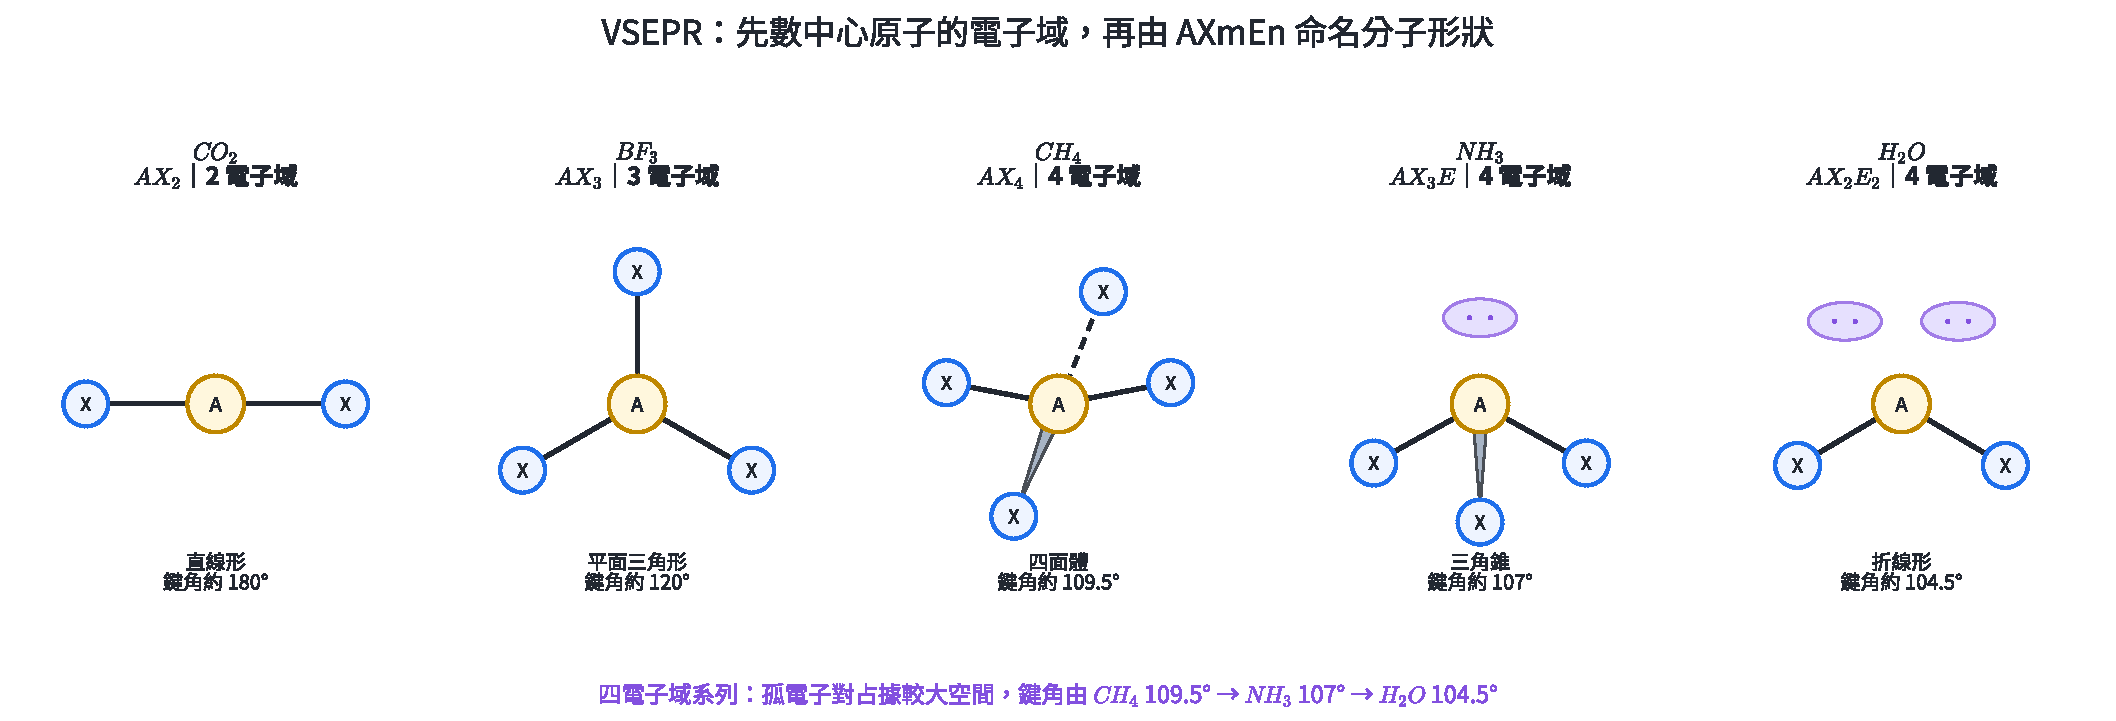
\includegraphics[width=0.99\linewidth,height=\textheight,keepaspectratio,alt={圖 7｜每個分子先讀 AX\_mE\_n 與電子域數，再核對鍵結域與孤電子對的總數。實楔表示鍵朝向觀察者，虛線表示鍵背向觀察者；四電子域系列的鍵角隨孤電子對增加而縮小。}]{assets/選化II-2-VSEPR電子域與分子形狀.pdf}
\caption{圖 7｜每個分子先讀 AX\(_m\)E\(_n\) 與電子域數，再核對鍵結域與孤電子對的總數。實楔表示鍵朝向觀察者，虛線表示鍵背向觀察者；四電子域系列的鍵角隨孤電子對增加而縮小。}
\end{figure}

\subsection{4.2 二至四電子域的核心形狀}\label{ux4e8cux81f3ux56dbux96fbux5b50ux57dfux7684ux6838ux5fc3ux5f62ux72c0}

{\def\LTcaptype{none} % do not increment counter
\begin{longtable}[]{@{}rllll@{}}
\toprule\noalign{}
總電子域 & 電子域幾何 & AX\(_m\)E\(_n\) & 分子形狀 & 代表例 \\
\midrule\noalign{}
\endhead
\bottomrule\noalign{}
\endlastfoot
2 & 直線 & AX\(_2\) & 直線 & CO\(_2\)、BeCl\(_2\) \\
3 & 平面三角 & AX\(_3\) & 平面三角 & BF\(_3\) \\
3 & 平面三角 & AX\(_2\)E & 折線 & SO\(_2\) \\
4 & 四面體 & AX\(_4\) & 四面體 & CH\(_4\) \\
4 & 四面體 & AX\(_3\)E & 三角錐 & NH\(_3\) \\
4 & 四面體 & AX\(_2\)E\(_2\) & 折線 & H\(_2\)O \\
\end{longtable}
}

孤電子對只受一個原子核吸引，電子雲較向外展開，通常占據較大空間；排斥量級為

\[
\text{孤—孤}>\text{孤—鍵}>\text{鍵—鍵}.
\]

因此同為四電子域時，鍵角常呈

\[
\angle\mathrm{HCH}=109.5^\circ>
\angle\mathrm{HNH}\approx107^\circ>
\angle\mathrm{HOH}\approx104.5^\circ.
\]

多鍵算一個電子域，但其電子密度通常比單鍵寬廣，對鄰域排斥稍強；若題目提供實測鍵角，應用此差異解釋偏離理想角。

\subsection{4.3 判斷流程}\label{ux5224ux65b7ux6d41ux7a0b}

\begin{enumerate}
\def\labelenumi{\arabic{enumi}.}
\tightlist
\item
  畫出合理 Lewis 結構，核對價電子總數與形式電荷。
\item
  選定中心原子，數成鍵方向 \(m\) 與中心孤電子對 \(n\)。
\item
  以 \(m+n\) 決定電子域幾何。
\item
  用 AX\(_m\)E\(_n\) 去除孤電子對位置，命名分子形狀。
\item
  由孤電子對與多鍵的排斥修正鍵角趨勢。
\end{enumerate}

理解用：五電子域可形成三角雙錐，六電子域可形成八面體；其孤電子對位置還需區分赤道與軸向。本章計算與主要練習聚焦二至四電子域，五、六電子域只在題目明示幾何時使用。

\begin{HandoutWorkedExample}

\subsection{\texorpdfstring{示範 9｜由 Lewis 結構判斷 NH\(_3\) 與 H\(_2\)O}{示範 9｜由 Lewis 結構判斷 NH\_3 與 H\_2O}}\label{ux793aux7bc4-9ux7531-lewis-ux7d50ux69cbux5224ux65b7-nh_3-ux8207-h_2o}

NH\(_3\) 的中心 N 有三個 N---H 成鍵域與一對孤電子：

\[
\mathrm{AX_3E},\qquad m+n=4.
\]

電子域幾何為四面體；去除孤電子對位置後，三個 H 形成三角錐。孤---鍵排斥較強，H---N---H 約 \(107^\circ\)。

H\(_2\)O 的中心 O 有兩個 O---H 成鍵域與兩對孤電子：

\[
\mathrm{AX_2E_2},\qquad m+n=4.
\]

電子域幾何同樣為四面體；兩個 H 的核位置形成折線。兩對孤電子造成更大的壓縮，H---O---H 約 \(104.5^\circ\)。因此電子域數相同不保證分子形狀或鍵角相同。

\end{HandoutWorkedExample}

\begin{HandoutWorkedExample}

\subsection{示範 10｜多鍵只算一個電子域}\label{ux793aux7bc4-10ux591aux9375ux53eaux7b97ux4e00ux500bux96fbux5b50ux57df}

甲醛 \(\mathrm{H_2C=O}\) 的中心碳與兩個 H、一个 O 相連。C=O 雙鍵雖含一個 \(\sigma\) 與一個 \(\pi\)，在空間中仍指向同一個 O，因此算一個電子域。

中心 C 的電子域為

\[
2(\mathrm{C-H})+1(\mathrm{C=O})=3,
\]

無孤電子對，所以是 AX\(_3\)、平面三角形，中心碳附近原子近似共平面。C=O 電子密度較大，對兩側 C---H 域排斥較強，因此實測 H---C---H 角可略小於理想 \(120^\circ\)。

\end{HandoutWorkedExample}

\begin{HandoutWorkedExample}

\subsection{示範 11｜由形狀資料反推孤電子對數}\label{ux793aux7bc4-11ux7531ux5f62ux72c0ux8cc7ux6599ux53cdux63a8ux5b64ux96fbux5b50ux5c0dux6578}

某 AX\(_3\) 分子的三個 X 不共平面，X---A---X 鍵角約 \(107^\circ\)。判斷中心原子的電子域與孤電子對數。

三個相連原子若沒有孤電子對，AX\(_3\) 的三電子域應為平面三角、約 \(120^\circ\)。資料顯示三角錐且角度接近 NH\(_3\)，因此中心另有一個孤電子域：

\[
\mathrm{AX_3E},\qquad 4\text{ 電子域},\qquad n=1.
\]

三維形狀與鍵角共同提供證據；只看化學式中的三個 X 會漏掉孤電子對。

\end{HandoutWorkedExample}

\subsection{4.4 直接用途}\label{ux76f4ux63a5ux7528ux9014-1}

分子形狀控制受體與藥物能否在三維空間互補，也控制液晶分子的排列、催化劑反應位點與材料偶極方向。VSEPR 能快速提供主族小分子的第一層幾何；精確鍵角、過渡金屬配位幾何與離域電子系統需由光譜、繞射與量子化學補充。

\subsection{練習 4}\label{ux7df4ux7fd2-4}

\begin{enumerate}
\def\labelenumi{\arabic{enumi}.}
\tightlist
\item
  判斷 CO\(_2\)、BF\(_3\)、CH\(_4\) 的 AX\(_m\)E\(_n\)、電子域幾何與分子形狀。
\item
  判斷 SO\(_2\)（中心 S 有一對孤電子）與 H\(_2\)O 的 AX\(_m\)E\(_n\)、分子形狀；說明兩者都是折線但電子域數不同。
\item
  將 CH\(_4\)、NH\(_3\)、H\(_2\)O 的鍵角由大到小排序，寫出排斥依據。
\item
  \(\mathrm{NO_3^-}\) 的任一共振式在中心 N 周圍有三個成鍵方向、無孤電子對。判斷中心幾何與所有原子是否近似共平面。
\item
  \(\mathrm{CH_3^+}\) 的中心碳有三個成鍵域、無孤電子；\(\mathrm{CH_3^-}\) 有三個成鍵域、一對孤電子。分別判斷形狀與理想角度趨勢。
\item
  某分子中心為 AX\(_2\)E，實測 X---A---X 小於 \(120^\circ\)。由電子域幾何與孤電子對排斥說明此結果。
\end{enumerate}

\subsection{練習 4 解析}\label{ux7df4ux7fd2-4-ux89e3ux6790}

\begin{enumerate}
\def\labelenumi{\arabic{enumi}.}
\tightlist
\item
  CO\(_2\)：AX\(_2\)，直線電子域、直線分子；BF\(_3\)：AX\(_3\)，平面三角電子域、平面三角分子；CH\(_4\)：AX\(_4\)，四面體電子域、四面體分子。
\item
  SO\(_2\)：AX\(_2\)E，共三電子域，電子域幾何平面三角，分子折線。H\(_2\)O：AX\(_2\)E\(_2\)，共四電子域，電子域幾何四面體，分子折線。相同形狀名稱不代表相同電子域幾何。
\item
  CH\(_4\) \(109.5^\circ>\) NH\(_3\) 約 \(107^\circ>\) H\(_2\)O 約 \(104.5^\circ\)。孤電子對數增加，孤---鍵與孤---孤排斥壓縮鍵角。
\item
  三電子域、無孤電子，為 AX\(_3\) 平面三角；N 與三個 O 近似共平面。共振改變鍵級分布的描述，不改變三個成鍵方向。
\item
  \(\mathrm{CH_3^+}\) 是 AX\(_3\) 平面三角，約 \(120^\circ\)；\(\mathrm{CH_3^-}\) 是 AX\(_3\)E 三角錐，電子域為四面體，鍵角小於 \(109.5^\circ\)。
\item
  AX\(_2\)E 的三個電子域先採平面三角排列，理想域角 \(120^\circ\)。孤電子對占據較大空間，對兩個成鍵域排斥較強，使 X---A---X 被壓縮到小於 \(120^\circ\)。
\end{enumerate}

\section{5. 鍵極性與分子極性}\label{ux9375ux6975ux6027ux8207ux5206ux5b50ux6975ux6027}

\subsection{5.1 電負度、部分電荷與鍵偶極}\label{ux96fbux8ca0ux5ea6ux90e8ux5206ux96fbux8377ux8207ux9375ux5076ux6975}

\textbf{電負度}描述原子在共價鍵中吸引共用電子的相對能力。兩原子電負度不同時，共用電子密度偏向電負度較大的原子，形成\textbf{極性共價鍵}。電荷偏移以部分電荷表示：

\[
\mathrm H^{\delta+}\!-\!\mathrm{Cl}^{\delta-}.
\]

鍵偶極矩的量級為

\[
\mu=qr,
\]

其中 \(q\) 是分離的部分電荷量級，\(r\) 是電荷中心距離。化學鍵偶極箭頭由 \(\delta+\) 指向 \(\delta-\)；箭尾的短橫標示正端。偶極矩常用德拜（D）表示，是向量而非只有大小的標量。

電負度差可用來比較同類鍵的極性趨勢。化學鍵從非極性共價、極性共價到高度離子性是一個連續光譜；單一差值界線只提供近似分類。

\subsection{5.2 分子偶極是所有鍵偶極的向量和}\label{ux5206ux5b50ux5076ux6975ux662fux6240ux6709ux9375ux5076ux6975ux7684ux5411ux91cfux548c}

分子偶極矩為各鍵偶極及孤電子對造成的電荷分布之向量合成：

\[
\vec\mu_{\mathrm{mol}}=\sum_i\vec\mu_i.
\]

因此「含極性鍵」不等於「分子必為極性」。先由 VSEPR 判斷三維形狀，再合成向量：

\begin{itemize}
\tightlist
\item
  CO\(_2\) 為直線形，兩個等大反向 C=O 鍵偶極相消，\(\vec\mu_{\mathrm{mol}}=0\)。
\item
  BF\(_3\) 為平面三角形，三個等大、相隔 \(120^\circ\) 的 B---F 鍵偶極相消。
\item
  H\(_2\)O 為折線形，兩個 O---H 鍵偶極不能相消，向量和沿 H---O---H 角平分線指向 O。
\item
  NH\(_3\) 為三角錐，三個 N---H 鍵偶極的合向量沿分子對稱軸，分子有極性。
\end{itemize}

\begin{figure}
\centering
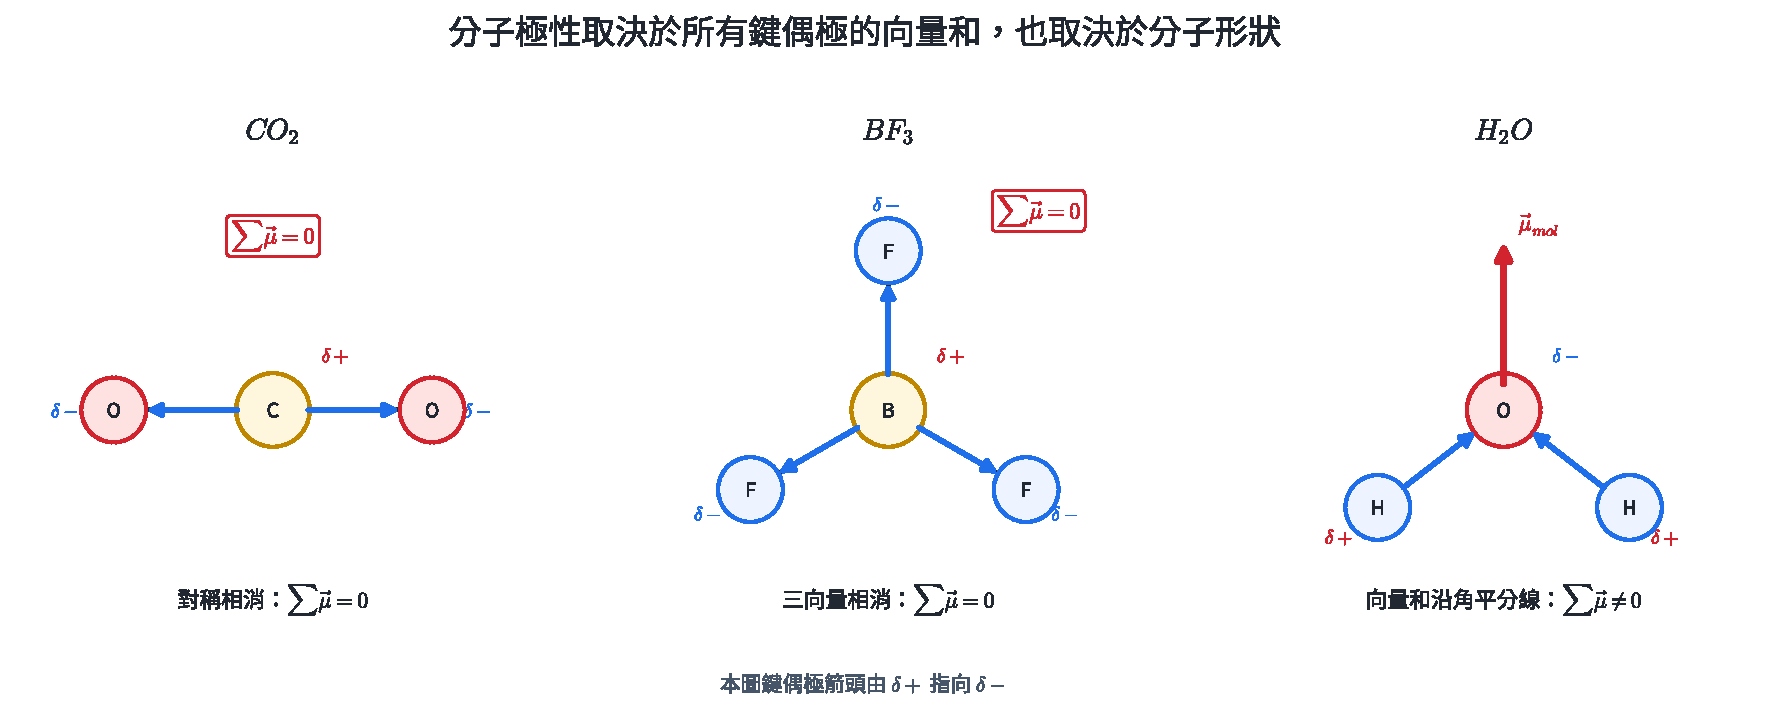
\includegraphics[width=0.97\linewidth,height=\textheight,keepaspectratio,alt={圖 8｜藍箭頭是各鍵偶極，方向由 \textbackslash delta+ 指向 \textbackslash delta-；紅箭頭是分子偶極向量和。CO\_2、BF\_3 的對稱使總和為零，H\_2O 的兩個 H---O 鍵偶極都指向 O，向量和沿鍵角平分線。}]{assets/選化II-2-鍵偶極向量和.pdf}
\caption{圖 8｜藍箭頭是各鍵偶極，方向由 \(\delta+\) 指向 \(\delta-\)；紅箭頭是分子偶極向量和。CO\(_2\)、BF\(_3\) 的對稱使總和為零，H\(_2\)O 的兩個 H---O 鍵偶極都指向 O，向量和沿鍵角平分線。}
\end{figure}

對稱相消需同時滿足「幾何位置對稱」與「向量大小相等」。CH\(_3\)Cl 的四面體骨架雖有高度對稱的母型，但一個 Cl 取代 H 後，四個鍵偶極不再等價，分子仍有極性。

\subsection{5.3 由電場觀察極性}\label{ux7531ux96fbux5834ux89c0ux5bdfux6975ux6027}

極性分子置於不均勻電場時，偶極會受到轉向與淨吸引。可用帶電塑膠梳靠近細水流：觀察是「水流向梳子偏折」；推論是「水分子的永久偶極在電場中重新取向，靠近梳子的一端受力較強」。

操作時以乾燥塑膠梳摩擦毛料，水流保持細且穩定，梳子不接觸水；讓插座與電器遠離水槽，完成後擦乾地面。這個觀察支持水可被電場取向，不能單靠偏折量直接求單分子偶極矩，因為流速、距離、電荷量與空氣濕度也會改變結果。

\begin{HandoutWorkedExample}

\subsection{\texorpdfstring{示範 12｜比較 CO\(_2\) 與 SO\(_2\) 的分子極性}{示範 12｜比較 CO\_2 與 SO\_2 的分子極性}}\label{ux793aux7bc4-12ux6bd4ux8f03-co_2-ux8207-so_2-ux7684ux5206ux5b50ux6975ux6027}

兩者都有極性鍵。CO\(_2\) 中心 C 是 AX\(_2\)，分子直線；兩個等大 C=O 偶極反向相消，所以 CO\(_2\) 為非極性分子。

SO\(_2\) 中心 S 是 AX\(_2\)E，分子折線；兩個 S---O 偶極的水平分量可互相抵消，沿角平分線的分量同向相加，所以總偶極不為零，SO\(_2\) 為極性分子。

差異來自中心孤電子對改變幾何，進而改變向量和；完整比較需同時納入鍵種類與分子形狀。

\end{HandoutWorkedExample}

\begin{HandoutWorkedExample}

\subsection{示範 13｜用向量分量求折線分子的總偶極}\label{ux793aux7bc4-13ux7528ux5411ux91cfux5206ux91cfux6c42ux6298ux7ddaux5206ux5b50ux7684ux7e3dux5076ux6975}

某 AX\(_2\) 折線分子有兩個等大的鍵偶極，每個為 \(1.50\ \mathrm D\)，夾角 \(104.5^\circ\)。求總偶極大小。

合向量沿角平分線。每個向量與角平分線夾角為 \(52.25^\circ\)；垂直分量相消，平行分量相加：

\[
\mu_{\mathrm{mol}}
=2(1.50)\cos52.25^\circ
=1.84\ \mathrm D.
\]

結果介於 \(0\) 與兩向量最大和 \(3.00\ \mathrm D\) 之間，符合幾何。這個計算假設兩個鍵偶極大小相同，且忽略更細緻的孤電子對貢獻。

\end{HandoutWorkedExample}

\begin{HandoutWorkedExample}

\subsection{示範 14｜四面體分子是否會相消}\label{ux793aux7bc4-14ux56dbux9762ux9ad4ux5206ux5b50ux662fux5426ux6703ux76f8ux6d88}

比較 CF\(_4\) 與 CH\(_3\)F。

CF\(_4\) 的四個 C---F 鍵等價，沿四面體四個頂點方向；對稱性使向量和為零，所以 CF\(_4\) 非極性。

CH\(_3\)F 仍為四面體，但三個 C---H 與一個 C---F 的偶極大小、方向角色不同，已失去四個等向量的完全對稱。向量和不為零，且主要朝 F 端，因此 CH\(_3\)F 為極性。

判斷順序是「形狀 → 等價鍵組 → 向量和」，而非只看中心原子混成。

\end{HandoutWorkedExample}

\subsection{5.4 直接用途}\label{ux76f4ux63a5ux7528ux9014-2}

微波爐的交變電場使極性分子與離子響應並耗散能量；液晶顯示器利用具有方向性與偶極的分子在電場中改變排列；紅外光譜的振動是否吸收紅外光，取決於振動過程是否改變偶極矩。實際介電加熱還受頻率、導電度與材料損耗影響，分子極性提供第一層機制。

\subsection{練習 5}\label{ux7df4ux7fd2-5}

\begin{enumerate}
\def\labelenumi{\arabic{enumi}.}
\tightlist
\item
  以電負度判斷 H---F、H---Cl、Cl---Cl 的鍵偶極方向；哪一個必為零？
\item
  判斷 BeCl\(_2\)、BF\(_3\)、NH\(_3\)、H\(_2\)O 的分子形狀與極性。
\item
  CO\(_2\) 與 HCN 都是直線形。說明前者非極性、後者極性的向量原因。
\item
  某折線 AX\(_2\) 的兩鍵偶極皆為 \(2.00\ \mathrm D\)，夾角 \(120^\circ\)。求總偶極大小。
\item
  判斷 CCl\(_4\) 與 CHCl\(_3\) 的極性，指出「四面體」資訊為何仍不足以直接作答。
\item
  帶電梳使細水流偏折。分別寫出一項直接觀察、一項粒子模型推論與一項會影響偏折量的控制變因。
\end{enumerate}

\subsection{練習 5 解析}\label{ux7df4ux7fd2-5-ux89e3ux6790}

\begin{enumerate}
\def\labelenumi{\arabic{enumi}.}
\item
  F、Cl 的電負度都大於 H，H---F 與 H---Cl 偶極分別由 H 指向 F、Cl；Cl---Cl 兩端相同，鍵偶極為零。
\item
  BeCl\(_2\)：直線，兩等大鍵偶極相消，非極性。BF\(_3\)：平面三角，三向量相消，非極性。NH\(_3\)：三角錐，向量和不為零，極性。H\(_2\)O：折線，向量和不為零，極性。
\item
  CO\(_2\) 兩個等大反向 C=O 偶極相消；HCN 兩端原子不同，H---C 與 C\(\equiv\)N 偶極不構成等大反向的一組，總偶極不為零。
\item
  \[
  \mu=2(2.00)\cos60^\circ=2.00\ \mathrm D.
  \]
\item
  CCl\(_4\) 四個鍵等價並沿四面體對稱方向，向量和為零；CHCl\(_3\) 有三個 C---Cl 與一個 C---H，向量大小不全相等，總和不為零。形狀只給方向，還需鍵偶極大小與取代基是否等價。
\item
  觀察：水流朝梳子方向偏折。推論：水偶極在不均勻電場中取向並受到淨吸引。控制變因可為梳子---水流距離、摩擦次數、水流速率或空氣濕度；比較時固定其中其餘變因。
\end{enumerate}

\section{6. 分子間的作用力}\label{ux5206ux5b50ux9593ux7684ux4f5cux7528ux529b}

\subsection{6.1 分子內鍵與分子間力的尺度}\label{ux5206ux5b50ux5167ux9375ux8207ux5206ux5b50ux9593ux529bux7684ux5c3aux5ea6}

\textbf{分子內鍵}把原子連成同一分子；\textbf{分子間作用力}存在於不同分子或粒子之間。液體沸騰時，分子彼此分離但分子式通常不變，因此主要克服分子間作用力。把水煮成水蒸氣不會大量切斷 O---H 共價鍵。

所有原子與分子都有電子雲，因此都有分散力；有永久偶極的分子還有偶極---偶極力；具適當供體與受體時，另可形成氫鍵。實際物質同時存在多種作用，所謂「主要作用力」是為了在受控比較中找出主導差異。

\begin{figure}
\centering
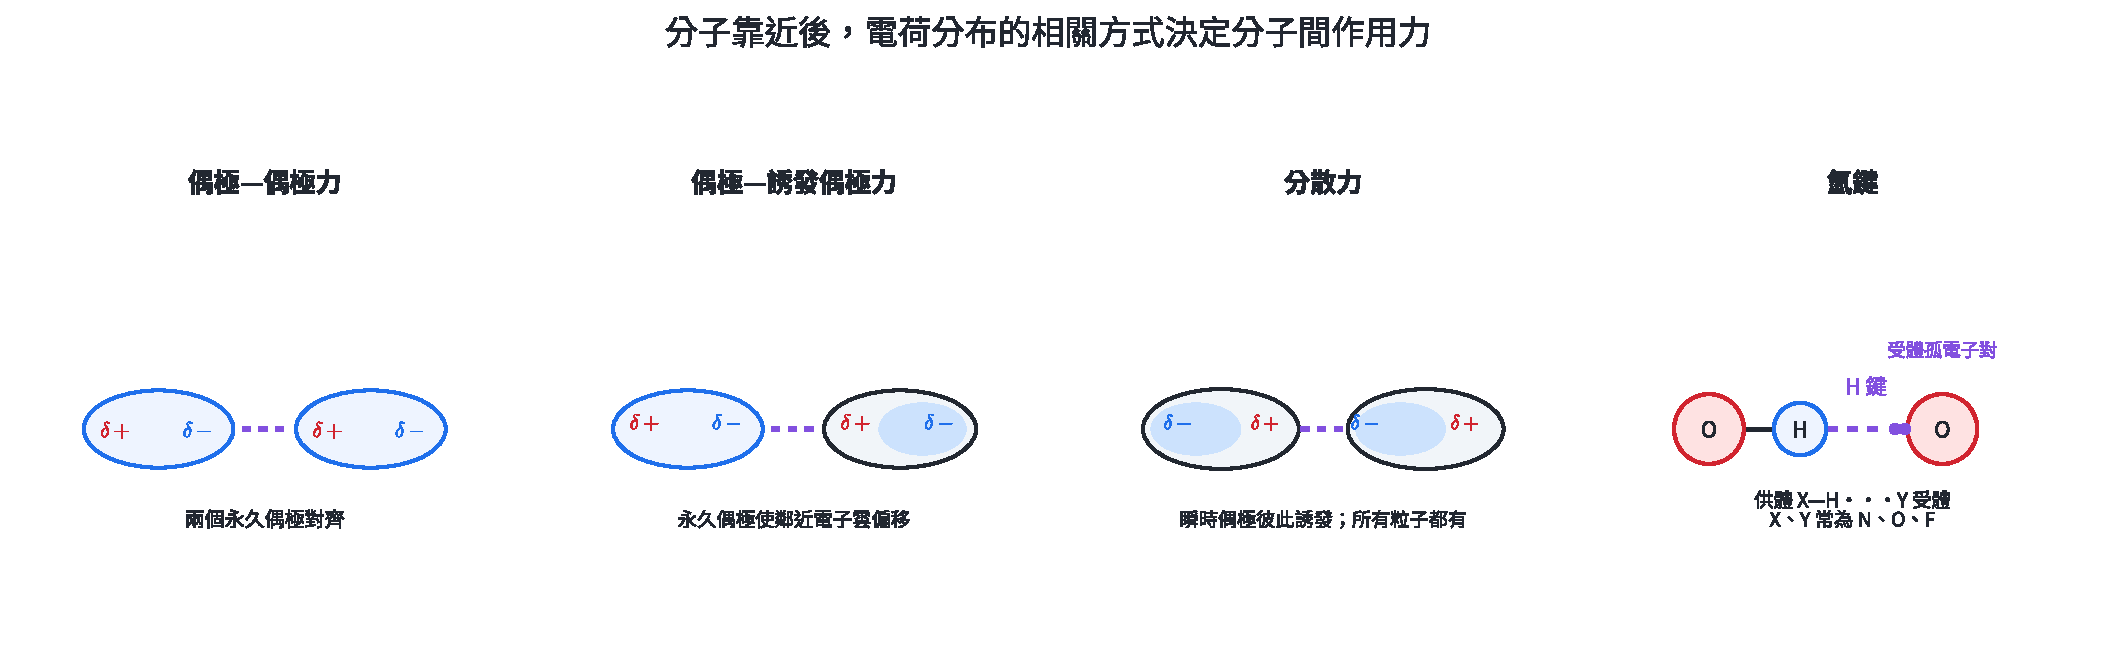
\includegraphics[width=0.99\linewidth,height=\textheight,keepaspectratio,alt={圖 9｜由左至右比較永久偶極、被誘發電子偏移、瞬時偶極相關與 X---H···Y 氫鍵。每個面板的虛線都連接實際互相吸引的區域；氫鍵面板同時標出受體的孤電子對。}]{assets/選化II-2-分子間作用力.pdf}
\caption{圖 9｜由左至右比較永久偶極、被誘發電子偏移、瞬時偶極相關與 X---H···Y 氫鍵。每個面板的虛線都連接實際互相吸引的區域；氫鍵面板同時標出受體的孤電子對。}
\end{figure}

\subsection{6.2 偶極---偶極力與偶極---誘發偶極力}\label{ux5076ux6975ux5076ux6975ux529bux8207ux5076ux6975ux8a98ux767cux5076ux6975ux529b}

兩個極性分子的永久偶極相互取向，異號部分電荷靠近而降低位能，稱為\textbf{偶極---偶極力}。液態分子的熱運動使排列持續改變；統計平均後仍有淨吸引。

極性分子的永久偶極靠近非極性分子時，電場使非極性分子的電子雲相對原子核偏移，產生\textbf{誘發偶極}，兩者形成偶極---誘發偶極力。電子雲越大、越容易變形，稱為\textbf{極化率}越大，誘發作用通常越強。

\subsection{6.3 分散力}\label{ux5206ux6563ux529b}

任一粒子的電子位置會瞬時波動，形成\textbf{瞬時偶極}；它使鄰近粒子的電子雲產生相關偏移，形成吸引，稱為\textbf{倫敦分散力}。分散力存在於所有粒子，包括非極性分子與單原子稀有氣體。

在形狀相近的一系列分子中，電子數與電子雲體積增加，極化率通常增大，分散力增強，沸點上升。在分子式相同的異構物中，細長分子可有較大的接觸面積，分散作用通常比緊密球狀分子強。

\subsection{6.4 氫鍵的供體與受體}\label{ux6c2bux9375ux7684ux4f9bux9ad4ux8207ux53d7ux9ad4}

當 H 與高電負度且體積小的 N、O、F 直接共價相連時，H 端帶明顯 \(\delta+\)；它可與另一個 N、O、F 上可接近的孤電子對形成較強、具方向性的\textbf{氫鍵}：

\[
\mathrm{X-H\cdots Y},\qquad X,Y\in\{\mathrm N,\mathrm O,\mathrm F\}.
\]

\begin{itemize}
\tightlist
\item
  \textbf{供體}提供 X---H 鍵。
\item
  \textbf{受體}提供可接近的孤電子對。
\item
  X---H\(\cdots\)Y 越接近直線，重疊與靜電穩定通常越佳。
\end{itemize}

乙醇同時能供、受氫鍵；二甲醚的 O 能受氫鍵，但分子內沒有 O---H，純二甲醚不能彼此形成 O---H\(\cdots\)O 網路；NH\(_4^+\) 可供氫鍵，但正電 N 沒有孤電子對可作受體。

同一分子內若幾何允許，供體與受體也可形成\textbf{分子內氫鍵}。它會占用受體並改變分子形狀，使與其他分子形成氫鍵的能力降低；對沸點與溶解性的影響需連同整體結構判斷。

\subsection{6.5 由結構比較沸點}\label{ux7531ux7d50ux69cbux6bd4ux8f03ux6cb8ux9ede}

沸點是在液體蒸氣壓等於外壓時的溫度。相同外壓下，液相分子間吸引越強，通常需更高溫才有足夠分子進入氣相，沸點越高。比較順序可整理為：

\begin{enumerate}
\def\labelenumi{\arabic{enumi}.}
\tightlist
\item
  是否形成廣泛離子作用或氫鍵網路。
\item
  分子永久偶極與可形成的供受體數。
\item
  電子雲大小與極化率。
\item
  分子形狀、接觸面積與支鏈程度。
\end{enumerate}

\begin{figure}
\centering
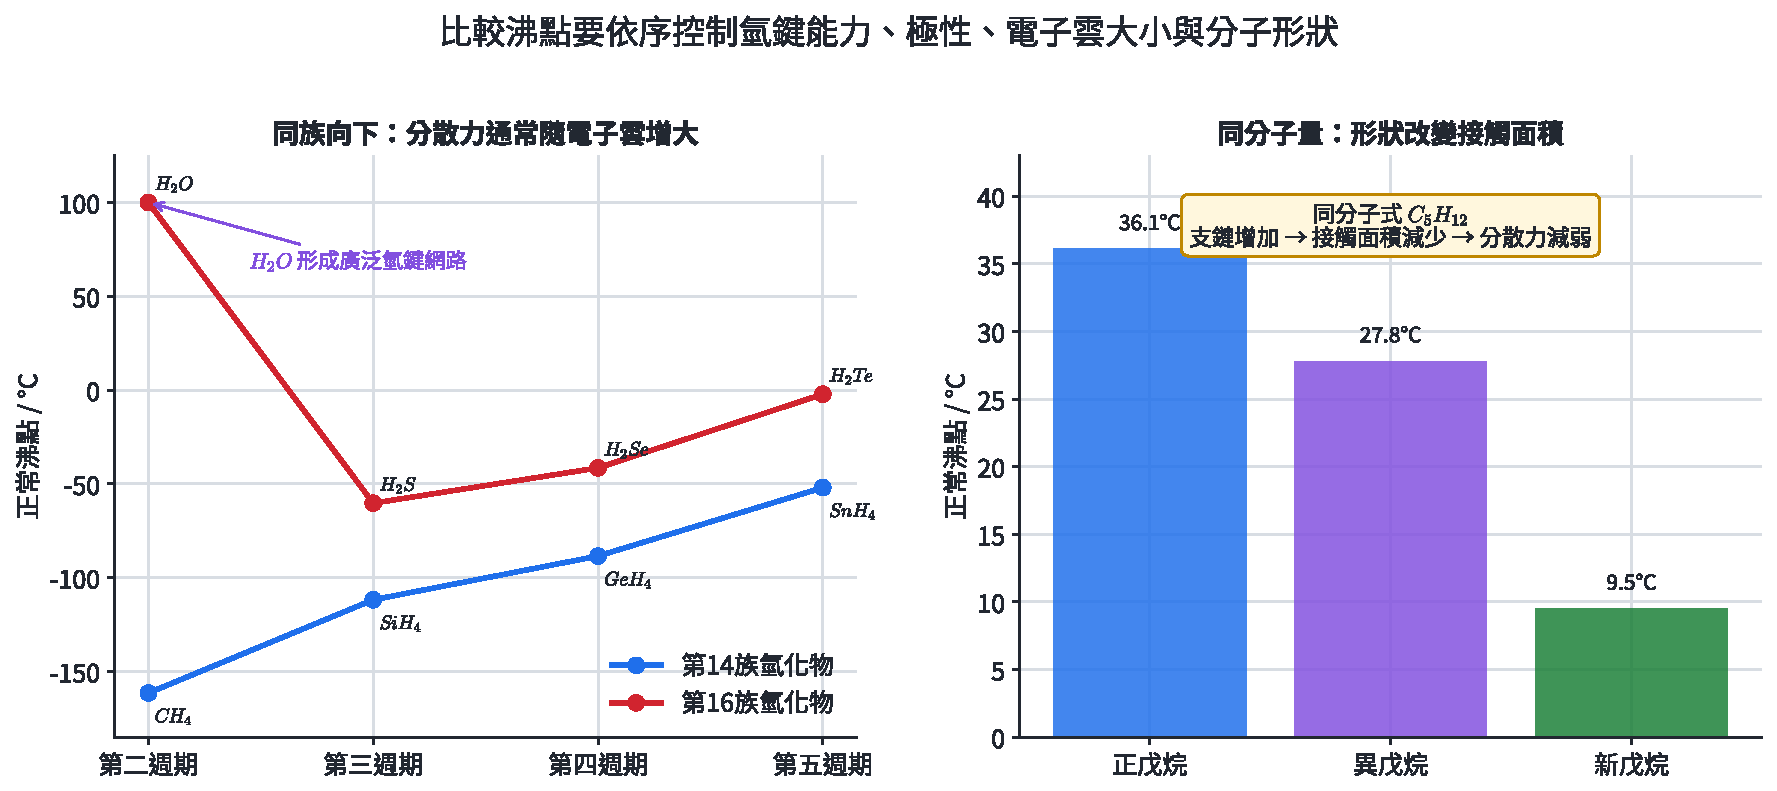
\includegraphics[width=0.98\linewidth,height=\textheight,keepaspectratio,alt={圖 10｜左圖以同族氫化物分離「電子雲變大」與水的氫鍵異常；右圖控制同分子式，顯示支鏈增加時戊烷異構物沸點下降。}]{assets/選化II-2-沸點資料與分子結構.pdf}
\caption{圖 10｜左圖以同族氫化物分離「電子雲變大」與水的氫鍵異常；右圖控制同分子式，顯示支鏈增加時戊烷異構物沸點下降。}
\end{figure}

「相似相溶」可用作用力與能量更精確表述：溶解需分開溶質粒子與溶劑分子，並建立新的溶質---溶劑作用。新作用足以補償原有作用，且混合帶來的熵效應有利時，溶解較容易。水可用離子---偶極作用水合離子，也可與含 O---H、N---H 或孤電子對的分子形成氫鍵。

\begin{HandoutWorkedExample}

\subsection{\texorpdfstring{示範 15｜H\(_2\)O 與 H\(_2\)S 的沸點差}{示範 15｜H\_2O 與 H\_2S 的沸點差}}\label{ux793aux7bc4-15h_2o-ux8207-h_2s-ux7684ux6cb8ux9edeux5dee}

H\(_2\)O 與 H\(_2\)S 都是折線極性分子，都有偶極---偶極力與分散力。H\(_2\)O 的 O---H 可作氫鍵供體，O 的孤電子對可作受體，因此液態水形成廣泛氫鍵網路。H\(_2\)S 的 S 體積較大、電負度較低，不符合本章 N/O/F 氫鍵判準。

水的正常沸點約 \(100^\circ\mathrm C\)，H\(_2\)S 約 \(-60^\circ\mathrm C\)。H\(_2\)S 電子較多、分散力較強，仍不足以抵消水的氫鍵網路差異；這組資料的排序需先納入氫鍵，再比較莫耳質量。

\end{HandoutWorkedExample}

\begin{HandoutWorkedExample}

\subsection{示範 16｜戊烷異構物的沸點}\label{ux793aux7bc4-16ux620aux70f7ux7570ux69cbux7269ux7684ux6cb8ux9ede}

正戊烷、異戊烷與新戊烷分子式皆為 C\(_5\)H\(_{12}\)，電子數與莫耳質量相同，也都是非極性分子，主要差異是形狀。

正戊烷較細長，分子靠近時可有較大接觸面積；異戊烷較緊密；新戊烷最接近球狀。分散力平均依序減弱，因此正常沸點為

\[
36.1^\circ\mathrm C>27.8^\circ\mathrm C>9.5^\circ\mathrm C.
\]

這是控制分子式後的形狀效應；不同分子式比較時還需先處理氫鍵、極性與電子雲大小。

\end{HandoutWorkedExample}

\begin{HandoutWorkedExample}

\subsection{示範 17｜判斷氫鍵供受體與水溶性}\label{ux793aux7bc4-17ux5224ux65b7ux6c2bux9375ux4f9bux53d7ux9ad4ux8207ux6c34ux6eb6ux6027}

比較乙醇 CH\(_3\)CH\(_2\)OH、二甲醚 CH\(_3\)OCH\(_3\) 與乙烷 C\(_2\)H\(_6\)。

\begin{itemize}
\tightlist
\item
  乙醇：O---H 可供氫鍵，O 的孤電子對可受氫鍵；能與水形成多向氫鍵。
\item
  二甲醚：O 有孤電子對，可接受水的氫鍵；沒有 O---H，純物質彼此不能形成 O---H\(\cdots\)O 網路。
\item
  乙烷：沒有 N/O/F，也沒有永久偶極，與水主要只有較弱的分散與誘發作用。
\end{itemize}

三者都含分散力；在與水的混合中，乙醇與二甲醚能建立較強溶質---水作用，乙烷則較難補償破壞水---水氫鍵的代價。碳鏈變長時，非極性部分增大，醇的水溶性通常下降。

\end{HandoutWorkedExample}

\subsection{6.6 直接用途與資料邊界}\label{ux76f4ux63a5ux7528ux9014ux8207ux8cc7ux6599ux908aux754c}

冷媒需在工作溫區易液化、易汽化，分子間作用力直接影響沸點；藥物的水溶性取決於離子化、氫鍵與疏水表面；DNA 鹼基配對與蛋白質二級結構利用多個方向性氫鍵共同穩定；燃料蒸氣壓與支鏈造成的沸點差會影響啟動與儲運。

沸點還受外壓影響，溶解度還受晶格能、溫度、酸鹼平衡與熵影響。分子間力提供機制主線；題目若給定外壓、相態或反應平衡資料，需一併納入。

\subsection{練習 6}\label{ux7df4ux7fd2-6}

\begin{enumerate}
\def\labelenumi{\arabic{enumi}.}
\tightlist
\item
  分別寫出 HCl---HCl、HCl---Ar、Ar---Ar 間除分散力外可有的作用；哪一組只有分散力？
\item
  判斷 NH\(_3\)、CH\(_3\)OH、CH\(_3\)OCH\(_3\)、CH\(_4\) 是否能在純物質分子間彼此形成氫鍵，並列出供體、受體。
\item
  將 CH\(_4\)、SiH\(_4\)、GeH\(_4\) 的沸點由低到高排序，寫出極化率依據。
\item
  正丁烷與異丁烷同為 C\(_4\)H\(_{10}\)。預測何者沸點較高，說明接觸面積與分散力。
\item
  乙醇的沸點高於分子量相近的二甲醚。以純物質中的氫鍵網路說明；兩者都具備的作用力也要列出。
\item
  水能溶解 NaCl。用「分開原有粒子---建立新作用」描述過程，指出新形成的主要作用力。
\end{enumerate}

\subsection{練習 6 解析}\label{ux7df4ux7fd2-6-ux89e3ux6790}

\begin{enumerate}
\def\labelenumi{\arabic{enumi}.}
\tightlist
\item
  HCl---HCl 有偶極---偶極力；HCl---Ar 有偶極---誘發偶極力；Ar---Ar 只有分散力。三組都同時有分散力。
\item
  NH\(_3\)：N---H 供體、N 孤電子對受體，可彼此氫鍵。CH\(_3\)OH：O---H 供體、O 孤電子對受體，可彼此氫鍵。CH\(_3\)OCH\(_3\) 只有 O 受體、沒有 O---H/N---H/F---H 供體，純物質不能彼此形成本章定義的氫鍵。CH\(_4\) 無供體與受體。
\item
  CH\(_4<\)SiH\(_4<\)GeH\(_4\)。同族向下電子數與電子雲體積增加，極化率與分散力通常增大，沸點上升。
\item
  正丁烷較細長，平均接觸面積較大，分散力較強，因此沸點通常高於較緊密的異丁烷。
\item
  兩者都有分散力，也都有永久偶極造成的偶極---偶極力。乙醇同時有 O---H 供體與 O 受體，可形成延伸的氫鍵網路；二甲醚缺少供體，純物質無法建立同類網路，所以乙醇沸點較高。
\item
  溶解需分開 Na\(^+\)、Cl\(^-\) 的部分晶格作用，也需重排部分水---水氫鍵；水分子以 O 的負端朝 Na\(^+\)、H 的正端朝 Cl\(^-\) 排列，建立離子---偶極作用並水合離子。新作用與混合效應使過程可進行。
\end{enumerate}

\section{7. 章末分層題}\label{ux7ae0ux672bux5206ux5c64ux984c}

\subsection{基礎與概念}\label{ux57faux790eux8207ux6982ux5ff5}

\begin{enumerate}
\def\labelenumi{\arabic{enumi}.}
\item
  四種固體 W、X、Y、Z 的性質如下：W 固態不導電、熔融導電；X 固態導電且可延展；Y 熔點低且不導電；Z 熔點高、不導電且極硬。依序判斷最可能的結構類型。
\item
  LiF 與 LiI 的離子電荷相同，最近鄰距離分別為 \(201\ \mathrm{pm}\) 與 \(305\ \mathrm{pm}\)。用 \(|z_+z_-|/r\) 求 LiF 與 LiI 靜電吸引量級之比，並預測晶格能大小。
\item
  求下列每個分子的 \(\sigma\)、\(\pi\) 鍵數：

  \begin{enumerate}
  \def\labelenumii{\arabic{enumii}.}
  \tightlist
  \item
    \(\mathrm{H_2C=O}\)；
  \item
    \(\mathrm{N\equiv C-C\equiv N}\)。
  \end{enumerate}
\item
  取 \(D(\mathrm{N\equiv N})=945\)、\(D(\mathrm{H-H})=436\)、\(D(\mathrm{N-H})=391\ \mathrm{kJ\,mol^{-1}}\)，用平均鍵能估算

  \[
  \mathrm{N_2(g)+3H_2(g)\rightarrow2NH_3(g)}
  \]

  的反應焓。
\item
  判斷 \(\mathrm{CH_3-C\equiv N}\) 中甲基碳、腈基碳與 N 的混成；再求整個分子的 \(\sigma\)、\(\pi\) 鍵數。
\item
  對 CH\(_4\)、NH\(_3\)、H\(_2\)O，分別寫出 AX\(_m\)E\(_n\)、分子形狀，並將鍵角由大到小排序。
\end{enumerate}

\subsection{資料與模型選擇}\label{ux8cc7ux6599ux8207ux6a21ux578bux9078ux64c7}

\begin{enumerate}
\def\labelenumi{\arabic{enumi}.}
\setcounter{enumi}{6}
\item
  三個 AX\(_2\) 分子的資料如下。判斷 P、Q、R 的形狀與極性。

  {\def\LTcaptype{none} % do not increment counter
  \begin{longtable}[]{@{}lrrr@{}}
  \toprule\noalign{}
  分子 & 中心孤電子對 & X---A---X & 兩個 A---X 鍵偶極是否等大 \\
  \midrule\noalign{}
  \endhead
  \bottomrule\noalign{}
  \endlastfoot
  P & 0 & \(180^\circ\) & 是 \\
  Q & 1 & \(118^\circ\) & 是 \\
  R & 0 & \(180^\circ\) & 否 \\
  \end{longtable}
  }
\item
  比較 BF\(_3\)、NF\(_3\) 的分子形狀與極性。兩者都含三個 F，為何結果不同？
\item
  某折線分子兩個鍵偶極皆為 \(1.20\ \mathrm D\)，夾角 \(90.0^\circ\)。以向量分量或餘弦定理求總偶極。
\item
  下列正常沸點資料為 CH\(_4\) \(-161.5^\circ\mathrm C\)、SiH\(_4\) \(-111.8^\circ\mathrm C\)、GeH\(_4\) \(-88.5^\circ\mathrm C\)、SnH\(_4\) \(-52.0^\circ\mathrm C\)。說明趨勢；再預測同為非極性的 CCl\(_4\) 與 CF\(_4\) 何者沸點較高。
\item
  三種 C\(_5\)H\(_{12}\) 異構物正常沸點為 \(36.1,27.8,9.5^\circ\mathrm C\)。把數值分配給正戊烷、異戊烷、新戊烷，並用同分子式控制下的形狀效應解釋。
\item
  對 HF、HCl、HBr、HI，H---X 鍵極性隨族向下減弱，但 HCl、HBr、HI 的沸點常隨分子量增加而升高；HF 又明顯高於同系列趨勢。分別指出控制後兩個趨勢的作用力。
\end{enumerate}

\subsection{跨節整合題}\label{ux8de8ux7bc0ux6574ux5408ux984c}

\begin{enumerate}
\def\labelenumi{\arabic{enumi}.}
\setcounter{enumi}{12}
\item
  材料 A 的熔點為 \(2850^\circ\mathrm C\)，固態不導電、熔融導電；材料 B 熔點極高、沿薄片導電、層間易滑動；材料 C 熔點為 \(-23^\circ\mathrm C\)，由非極性分子組成。回答：

  \begin{enumerate}
  \def\labelenumii{\arabic{enumii}.}
  \tightlist
  \item
    判斷 A、B、C 的結構類型。
  \item
    對 A 寫出載流子由固態到熔融態的改變。
  \item
    對 B 連接「碳的局部 \(sp^2\)」與層內導電。
  \item
    C 的低熔點主要克服哪一層級的作用？
  \end{enumerate}
\item
  丙酮的骨架為 \(\mathrm{CH_3-C(=O)-CH_3}\)。回答：

  \begin{enumerate}
  \def\labelenumii{\arabic{enumii}.}
  \tightlist
  \item
    判斷羰基 C、O 與兩個甲基 C 的混成。
  \item
    求整個分子的 \(\sigma\)、\(\pi\) 鍵數。
  \item
    判斷羰基 C 周圍的局部形狀與整個分子是否有極性。
  \item
    丙酮能接受水的氫鍵，卻不能在純丙酮中彼此形成 O---H\(\cdots\)O 氫鍵。以供受體說明。
  \end{enumerate}
\item
  三種第二週期氫化物資料如下：

  {\def\LTcaptype{none} % do not increment counter
  \begin{longtable}[]{@{}lrrr@{}}
  \toprule\noalign{}
  物質 & 中心電子域 & 中心孤電子對 & 正常沸點 / \(^\circ\mathrm C\) \\
  \midrule\noalign{}
  \endhead
  \bottomrule\noalign{}
  \endlastfoot
  CH\(_4\) & 4 & 0 & \(-161.5\) \\
  NH\(_3\) & 4 & 1 & \(-33.3\) \\
  H\(_2\)O & 4 & 2 & \(100.0\) \\
  \end{longtable}
  }

  \begin{enumerate}
  \def\labelenumii{\arabic{enumii}.}
  \tightlist
  \item
    寫出三者形狀與鍵角排序。
  \item
    判斷三者分子極性。
  \item
    以氫鍵供受體數與可形成網路的程度解釋沸點排序；同時說明 CH\(_4\) 仍具有哪種分子間力。
  \end{enumerate}
\item
  乙烷 C\(_2\)H\(_6\)、二甲醚 CH\(_3\)OCH\(_3\)、乙醇 CH\(_3\)CH\(_2\)OH 的電子數與莫耳質量相近，正常沸點依序約為 \(-88.6,-24.8,78.4^\circ\mathrm C\)。回答：

  \begin{enumerate}
  \def\labelenumii{\arabic{enumii}.}
  \tightlist
  \item
    求三者全部重原子的混成。
  \item
    判斷三者的分子極性。
  \item
    列出各純物質中的分子間作用力與氫鍵供受體。
  \item
    以「三者都有分散力，再加入極性與氫鍵差異」建立完整沸點排序。
  \end{enumerate}
\end{enumerate}

\section{8. 章末分層題完整解析}\label{ux7ae0ux672bux5206ux5c64ux984cux5b8cux6574ux89e3ux6790}

\begin{enumerate}
\def\labelenumi{\arabic{enumi}.}
\item
  W 固態離子固定、熔融後離子可移動，為離子晶體。X 有可移動電子且層滑移後仍維持金屬鍵，為金屬晶體。Y 低熔點且無載流子，為分子物質。Z 極硬、高熔點且不導電，最符合三維共價網狀固體。
\item
  電荷乘積相同，故

  \[
  \frac{S_{\mathrm{LiF}}}{S_{\mathrm{LiI}}}
  =\frac{1/201}{1/305}
  =\frac{305}{201}=1.52.
  \]

  LiF 的庫侖吸引量級約為 LiI 的 \(1.52\) 倍，預期 LiF 晶格能較大。精確值仍受晶格型式與排斥項影響。
\item
  \begin{enumerate}
  \def\labelenumii{\arabic{enumii}.}
  \tightlist
  \item
    H\(_2\)C=O 有兩個 C---H 相連對與一個 C---O 相連對，故 \(3\sigma\)；C=O 再給 \(1\pi\)。
  \item
    N\(\equiv\)C---C\(\equiv\)N 有三個相連對，故 \(3\sigma\)；兩個三鍵各有 \(2\pi\)，共 \(4\pi\)。
  \end{enumerate}
\item
  斷裂一個 N\(\equiv\)N 與三個 H---H，形成六個 N---H：

  \[
  \begin{aligned}
  \Delta H
  &\approx[945+3(436)]-6(391)\\
  &=2253-2346\\
  &=-93\ \mathrm{kJ\,mol^{-1}}.
  \end{aligned}
  \]

  以方程式所寫反應量為基準，估算為放熱 \(93\ \mathrm{kJ}\)。平均鍵能法未包含實際分子環境的全部差異。
\item
  甲基碳形成四個 \(\sigma\) 方向，為 \(sp^3\)。腈基碳與 N 形成三鍵，兩者各需保留兩個 \(p\) 形成兩個 \(\pi\)，故皆為 \(sp\)。相連對為三個 C---H、C---C、C---N，共 \(5\sigma\)；C\(\equiv\)N 給 \(2\pi\)。
\item
  CH\(_4\)：AX\(_4\)、四面體；NH\(_3\)：AX\(_3\)E、三角錐；H\(_2\)O：AX\(_2\)E\(_2\)、折線。三者皆四電子域，孤電子對數依序增加，故

  \[
  109.5^\circ>107^\circ>104.5^\circ.
  \]
\item
  P 無孤電子、AX\(_2\)，呈直線；兩鍵偶極等大反向相消，非極性。Q 有一孤電子，為 AX\(_2\)E、折線；等大鍵偶極不能相消，極性。R 是直線，但兩鍵偶極不等大，反向後仍有剩餘，極性。資料顯示幾何對稱與向量等大缺一不可。
\item
  BF\(_3\) 的 B 有三成鍵域、無孤電子，為 AX\(_3\) 平面三角；三個等大 B---F 向量相消，非極性。NF\(_3\) 的 N 有三成鍵域與一孤電子，為 AX\(_3\)E 三角錐；三個 N---F 向量不在同一平面相消，分子有極性。中心孤電子對造成的幾何差異改變了向量和。
\item
  兩向量等大且互成 \(90^\circ\)：

  \[
  \mu=\sqrt{(1.20)^2+(1.20)^2}
  =1.20\sqrt2
  =1.70\ \mathrm D.
  \]

  結果小於同向最大值 \(2.40\ \mathrm D\)，大於零，與折線幾何一致。
\item
  第 14 族氫化物皆近似非極性，向下電子數、電子雲體積與極化率增加，分散力增強，因此沸點依 CH\(_4<\)SiH\(_4<\)GeH\(_4<\)SnH\(_4\) 上升。CCl\(_4\) 與 CF\(_4\) 也都非極性且形狀相同；CCl\(_4\) 電子雲較大、極化率較高，預期沸點較高。
\item
  同分子式下，正戊烷最細長、接觸面積最大，分散力最強，配 \(36.1^\circ\mathrm C\)；異戊烷居中，配 \(27.8^\circ\mathrm C\)；新戊烷最緊密近球狀，接觸面積最小，配 \(9.5^\circ\mathrm C\)。
\item
  HCl、HBr、HI 不能形成強的 N/O/F---H 氫鍵；族向下電子雲增大，分散力增強，使沸點上升。HF 的 H---F 同時是氫鍵供體，F 的孤電子對是受體，液體可形成氫鍵網路，因此 HF 明顯高於只按分散力外推的趨勢。鍵極性大小本身不是這組沸點排序的唯一控制量。
\item
  \begin{enumerate}
  \def\labelenumii{\arabic{enumii}.}
  \tightlist
  \item
    A 固態不導電、熔融導電且熔點高，為離子晶體。B 層內導電、層間滑動，為石墨型層狀共價網狀固體。C 低熔點且由非極性分子構成，為分子物質。
  \item
    A 固態時正、負離子在晶格位置附近振動，無法長距離定向移動；熔融後晶格秩序破壞，離子可在電場中遷移而載流。
  \item
    B 中每個碳採 \(sp^2\)，三個混成軌域形成層內 \(\sigma\) 網路，剩餘一個垂直層面的 \(p\) 軌域彼此重疊，形成層內離域 \(\pi\) 電子，因此沿層面導電。
  \item
    C 熔化主要克服分子間作用力；因分子非極性，差異主要由分散力控制，不需大量切斷分子內共價鍵。
  \end{enumerate}
\item
  \begin{enumerate}
  \def\labelenumii{\arabic{enumii}.}
  \tightlist
  \item
    羰基 C 有三電子域並保留一個 \(p\) 形成 \(\pi\)，為 \(sp^2\)。羰基 O 同樣以一個未混成 \(p\) 形成 \(\pi\)，可用 \(sp^2\) 描述。兩個甲基 C 各有四個 \(\sigma\) 方向，為 \(sp^3\)。
  \item
    六個 C---H、兩個 C---C、一個 C---O 相連對，共 \(9\sigma\)；C=O 再有 \(1\pi\)。
  \item
    羰基 C 是 AX\(_3\)，局部平面三角。C=O 鍵偶極很大，兩側甲基無法生成等大反向向量抵消，因此整個丙酮分子有極性。
  \item
    丙酮 O 有孤電子對，可接受水的 O---H 氫鍵；丙酮本身沒有 O---H、N---H 或 F---H，缺少氫鍵供體，所以純丙酮分子間不能形成 O---H\(\cdots\)O 網路。純物質仍有偶極---偶極力與分散力。
  \end{enumerate}
\item
  \begin{enumerate}
  \def\labelenumii{\arabic{enumii}.}
  \tightlist
  \item
    CH\(_4\) 為 AX\(_4\) 四面體；NH\(_3\) 為 AX\(_3\)E 三角錐；H\(_2\)O 為 AX\(_2\)E\(_2\) 折線。孤電子對增加使鍵角依 CH\(_4>\)NH\(_3>\)H\(_2\)O 下降。
  \item
    CH\(_4\) 四個等價 C---H 向量沿四面體方向相消，視為非極性；NH\(_3\) 與 H\(_2\)O 的不對稱核位置使向量和不為零，皆為極性。
  \item
    CH\(_4\) 無 N/O/F---H 供體與受體，只有分散力，沸點最低。NH\(_3\) 每分子有 N---H 供體與一對可用孤電子對，可形成氫鍵，沸點升高。H\(_2\)O 有兩個 O---H 供體方向與兩對孤電子受體，可建立更廣泛的三維氫鍵網路，沸點最高。三者都有分散力，但此處氫鍵網路差異主導排序。
  \end{enumerate}
\item
  \begin{enumerate}
  \def\labelenumii{\arabic{enumii}.}
  \tightlist
  \item
    乙烷兩個 C 都是 \(sp^3\)。二甲醚兩個 C 各 \(sp^3\)，O 有兩鍵與兩孤電子域，也以 \(sp^3\) 描述。乙醇兩個 C 與 O 亦皆 \(sp^3\)。
  \item
    乙烷近似非極性；二甲醚的 C---O---C 為折線且 C---O 偶極不能相消，為極性；乙醇含極性 C---O、O---H 且結構不對稱，為極性。
  \item
    三者都有分散力。二甲醚與乙醇另有偶極---偶極力。二甲醚 O 是氫鍵受體但無供體，純物質不能彼此形成 O---H\(\cdots\)O 網路；乙醇 O 同時是受體，O---H 是供體，可彼此形成氫鍵。乙烷無供受體。
  \item
    三者電子數與莫耳質量相近，先控制分散力量級。乙烷無永久偶極，吸引最弱，沸點最低；二甲醚增加偶極---偶極力，沸點居中；乙醇再形成延伸氫鍵網路，分離分子需更多能量，沸點最高。因此 \(-88.6<-24.8<78.4^\circ\mathrm C\)。
  \end{enumerate}
\end{enumerate}

\section{9. 核心整理}\label{ux6838ux5fc3ux6574ux7406}

\begin{enumerate}
\def\labelenumi{\arabic{enumi}.}
\tightlist
\item
  鍵結穩定對應總位能最低點；平衡鍵長是最低點位置，鍵解離能是由最低點分離到遠處所需能量。
\item
  離子晶體由整個正負離子晶格的靜電作用穩定；比較量級時看 \(|z_+z_-|/r\)。金屬的離域電子同時解釋導電與延展。共價鍵有方向性；獨立分子與共價網狀固體的連接尺度不同。
\item
  單鍵、雙鍵、三鍵分別為 \(1\sigma\)、\(1\sigma+1\pi\)、\(1\sigma+2\pi\)。同種原子間鍵級增加時，鍵長通常縮短、總鍵能增加；\(\pi\) 鍵限制繞鍵軸轉動。
\item
  \(sp^3,sp^2,sp\) 分別產生 \(4,3,2\) 個混成軌域並留下 \(0,1,2\) 個未混成 \(p\)；軌域總數與電子總數守恆。
\item
  VSEPR 先數成鍵方向與中心孤電子對。多鍵算一域；分子形狀只由原子核位置命名。孤電子對排斥較強，使實際鍵角縮小。
\item
  鍵極性由電荷偏移產生；分子極性是所有鍵偶極的向量和。幾何對稱與向量等大同時成立時才會完全相消。
\item
  所有粒子都有分散力；極性分子另有偶極相關作用。氫鍵需 X---H 供體與 N/O/F 孤電子對受體。比較沸點時依序控制氫鍵、極性、極化率與形狀。
\item
  從性質反推結構時，使用多項獨立證據：熔點指出分離所需能量，固／液導電指出載流子可動性，硬度與延展指出連接方向，沸點與溶解則反映粒子間作用及環境條件。
\end{enumerate}


\end{document}
